 % The main file for CAMP reports
 % Don't put any content in here.
 % Don't even include content files by using \input or \inlcude.
 % Put your content to TEXT.TEX or include it there using \input.
 % Uses:
 %		SETTINGS.TEX	contains the settings for this document
 %		COMMANDS.TEX	contains commands which can be used while writing
 %		INFO.TEX			contains the author, title and so on for the cover
 %		COVER.TEX			formats the front cover of the document
 %		ABSTRACT.TEX	contains the abstract to be included (if needed)
 %		TEXT.TEX			contains the actual content of the document
 %		BIB.BIB				containt the BibTeX entries for the document


%% Draft document mode
%% Final document
\documentclass[11pt,a4paper,bibtotoc,idxtotoc,headsepline,footsepline,footexclude,BCOR14mm,DIV13]{scrbook}

%\documentclass[11pt,a4paper,bibtotoc,idxtotoc,headsepline,footsepline,footexclude,BCOR20mm,DIV10]{scrbook}

% KOMA-Optionen:
%  bibtotoc: include bibliography in table of contents
%  idxtotoc: include index in table of contents
%  headsepline: use horizontalline under heading
%  BCOR: binding correcion (Bindungskorrektur) (e.g.: BCOR5mm)
%  DIV: Number of sheet sections (used for layout) (e.g.: DIV12)



% include title and author information for the cover
% Set here the title, authors and other stuff to be used for the cover
% This file is used by MAIN.TEX

% set title, authors and stuff for the cover
\def\doctype{Bachelor's Thesis in Informatics}
\def\title{Reinforcement Learning for Path Planing of Robotic Arms}
\def\titleGer{Bestärkendes Lernen zur Pfadplanung von robotischen Armen}
\def\author{Anton Mai}
\def\date{February 17, 2020}

% text to appear in the footer
\def\footertext{}


% include settings
\PassOptionsToPackage{table,svgnames,dvipsnames}{xcolor}

\usepackage[utf8]{inputenc}
\usepackage[T1]{fontenc}
\usepackage[sc]{mathpazo}
\usepackage[ngerman,american]{babel}
\usepackage[autostyle]{csquotes}
\usepackage[%
  backend=biber,
  url=false,
  style=alphabetic,
  maxnames=4,
  minnames=3,
  maxbibnames=99,
  giveninits,
  uniquename=init]{biblatex} % TODO: adapt citation style
\usepackage{graphicx}
\usepackage{scrhack} % necessary for listings package
\usepackage{listings}
\usepackage{lstautogobble}
\usepackage{tikz}
\usepackage{pgfplots}
\usepackage{pgfplotstable}
\usepackage{booktabs}
\usepackage[final]{microtype}
\usepackage{caption}
\usepackage[hidelinks]{hyperref} % hidelinks removes colored boxes around references and links

\bibliography{bibliography}

\setkomafont{disposition}{\normalfont\bfseries} % use serif font for headings
\linespread{1.05} % adjust line spread for mathpazo font

% Add table of contents to PDF bookmarks
\BeforeTOCHead[toc]{{\cleardoublepage\pdfbookmark[0]{\contentsname}{toc}}}

% Define TUM corporate design colors
% Taken from http://portal.mytum.de/corporatedesign/index_print/vorlagen/index_farben
\definecolor{TUMBlue}{HTML}{0065BD}
\definecolor{TUMSecondaryBlue}{HTML}{005293}
\definecolor{TUMSecondaryBlue2}{HTML}{003359}
\definecolor{TUMBlack}{HTML}{000000}
\definecolor{TUMWhite}{HTML}{FFFFFF}
\definecolor{TUMDarkGray}{HTML}{333333}
\definecolor{TUMGray}{HTML}{808080}
\definecolor{TUMLightGray}{HTML}{CCCCC6}
\definecolor{TUMAccentGray}{HTML}{DAD7CB}
\definecolor{TUMAccentOrange}{HTML}{E37222}
\definecolor{TUMAccentGreen}{HTML}{A2AD00}
\definecolor{TUMAccentLightBlue}{HTML}{98C6EA}
\definecolor{TUMAccentBlue}{HTML}{64A0C8}

% Settings for pgfplots
\pgfplotsset{compat=newest}
\pgfplotsset{
  % For available color names, see http://www.latextemplates.com/svgnames-colors
  cycle list={TUMBlue\\TUMAccentOrange\\TUMAccentGreen\\TUMSecondaryBlue2\\TUMDarkGray\\},
}

% Settings for lstlistings
\lstset{%
  basicstyle=\ttfamily,
  columns=fullflexible,
  autogobble,
  keywordstyle=\bfseries\color{TUMBlue},
  stringstyle=\color{TUMAccentGreen}
}


% include commands
% Commands to be used within the TUM report document
% Included by MAIN.TEX
% Please include your own cool commands here. 
% Be only sure to comment it sufficiently so others can use it.

%-------------------------------------------------------------
%                      Own Commands
%-------------------------------------------------------------


%-------------------------------------------------------------
% math stuff -------------------------------------------------

% nice R, N, C
\newcommand{\nat}{\mathbb{N}}
\newcommand{\real}{\mathbb{R}}
\newcommand{\compl}{\mathbb{C}}



% norm
\newcommand{\norm}[1]{\left\| #1 \right\|}

% un demi
\newcommand{\half}{\frac{1}{2}}

% parantheses
\newcommand{\parenth}[1]{ \left( #1 \right) }
\newcommand{\bracket}[1]{ \left[ #1 \right] }
\newcommand{\accolade}[1]{ \left\{ #1 \right\} }
%\newcommand{\angle}[1]{ \left\langle  #1 \right\rangle }

% partial derivative: %#1 function, #2 which variable
% simple / single line version
\newcommand{\pardevS}[2]{ \delta_{#1} f(#2) }
% fraction version
\newcommand{\pardevF}[2]{ \frac{\partial #1}{\partial #2} }

% render vectors: 3 and 4 dimensional
\newcommand{\veciii}[3]{\left[ \begin{array}[h]{c} #1 \\ #2 \\ #3	\end{array} \right]}
\newcommand{\veciv}[4]{\left[ \begin{array}[h]{c} #1 \\ #2 \\ #3 \\ #4	\end{array} \right]}

% render matrices: 3  dimensional (arguments in row first order)
\newcommand{\matiii}[9]{\left[ \begin{array}[h]{ccc} #1 & #2 & #3 \\ #4 & #5 & #6 \\ #7 & #8 & #9	\end{array} \right]}
%DOESN'T WORK,DON'T KNOW WHY \newcommand{\mativ}[16]{\left[ \begin{array}[h]{cccc} #1 & #2 & #3 & #4 \\ #5 & #6 & #7 & #8 \\ #9 & #10 & #11 & #12 \\ #13 & #14 & #15 & #16 \end{array} \right]}


%-------------------------------------------------------------
%-------------------------------------------------------------


%-------------------------------------------------------------
% some abreviations ------------------------------------------
\newcommand{\Reg}{$^{\textregistered}$}
\newcommand{\reg}{$^{\textregistered}$ }
\newcommand{\Tm}{\texttrademark}
\newcommand{\tm}{\texttrademark~}
\newcommand {\bsl} {$\backslash$}

%-------------------------------------------------------------
%-------------------------------------------------------------


%-------------------------------------------------------------
% formating --------------------------------------------------

% Theorem & Co environments and counters
\newtheorem{theorem}{Theorem}[chapter]
\newtheorem{lemma}[theorem]{Lemma}
\newtheorem{corollary}[theorem]{Corollary}
\newtheorem{remark}[theorem]{Remark}
\newtheorem{definition}[theorem]{Definition}
\newtheorem{equat}[theorem]{Equation}
\newtheorem{example}[theorem]{Example}
\newtheorem{algorithm}[theorem]{Algorithm}

% inserting figures
\newcommand{\insertfigure}[4]{ % Filename, Caption, Label, Width percent of textwidth
	\begin{figure}[htbp]
		\begin{center}
			\includegraphics[width=#4\textwidth]{#1}
		\end{center}
		\vspace{-0.4cm}
		\caption{#2}
		\label{#3}
	\end{figure}
}




% referecing figures

\newcommand{\refFigure}[1]{ %label
	figure \ref{#1}
}
\newcommand{\refChapter}[1]{ %label
	chapter \ref{#1}
}

\newcommand{\refSection}[1]{ %label
	section \ref{#1}
}

\newcommand{\refParagraph}[1]{ %label
	paragraph \ref{#1}
}

\newcommand{\refEquation}[1]{ %label
	equation \ref{#1}
}

\newcommand{\refTable}[1]{ %label
	table \ref{#1}
}




\newcommand{\rigidTransform}[2]
{
	${}^{#2}\!\mathbf{H}_{#1}$
}

%code, in typewriter
\newcommand{\code}[1]
 {\texttt{#1}}

% comment that appears on the border - very practical !!!
\newcommand{\comment}[1]{\marginpar{\raggedright \noindent \footnotesize {\sl #1} }}

% page clearing
\newcommand{\clearemptydoublepage}{%
  \ifthenelse{\boolean{@twoside}}{\newpage{\pagestyle{empty}\cleardoublepage}}%
  {\clearpage}}


%-------------------------------------------------------------
%-------------------------------------------------------------


\newcommand{\etAl}{\emph{et al.}\mbox{ }}

\pdfinfo{
   /Author (Alexander Gillert)
   /Title (Direct GPU-FPGA Communication)
   /Keywords (FPGA, GPU, OpenCL, PCIe, DMA)
}

\hypersetup{%
pdftitle={Direct GPU-FPGA Communication},%
pdfauthor={Alexander Gillert},%
pdfkeywords={FPGA, GPU, OpenCL, PCIe, DMA},%
}%

\hypersetup{
    colorlinks=false,
    pdfborder={0 0 0},
}


%\makeindex
	%% inter line spacing
%\linespread{1.0}

\makeglossary

\begin{document}

	\frontmatter
	
	
	\begin{titlepage}
  % HACK for two-sided documents: ignore binding correction for cover page.
  % Adapted from Markus Kohm's KOMA-Script titlepage=firstiscover handling.
  % See http://mirrors.ctan.org/macros/latex/contrib/koma-script/scrkernel-title.dtx,
  % \maketitle macro.
  \oddsidemargin=\evensidemargin\relax
  \textwidth=\dimexpr\paperwidth-2\evensidemargin-2in\relax
  \hsize=\textwidth\relax

  \centering

  \IfFileExists{logos/tum.pdf}{%
    \includegraphics[height=20mm]{logos/tum.pdf}
  }{%
    \vspace*{20mm}
  }

  \vspace{5mm}
  {\huge\MakeUppercase{\getFaculty{}}}\\

  \vspace{5mm}
  {\large\MakeUppercase{\getUniversity{}}}\\

  \vspace{20mm}
  {\Large \getDoctype{}}

  \vspace{15mm}
  {\huge\bfseries \getTitle{}}

  \vspace{15mm}
  {\LARGE \getAuthor{}}

  \IfFileExists{logos/faculty.pdf}{%
    \vfill{}
    \includegraphics[height=20mm]{logos/faculty.pdf}
  }{}
\end{titlepage}

%	\clearemptydoublepage
%	
%	% The titlepage for the CAMP report document.
% Included by MAIN.TEX


%--------------------------------------------------
% The title page
%--------------------------------------------------

% correct BCOR - undo at the end !!!
\def\bcorcor{0.15cm}
\addtolength{\hoffset}{\bcorcor}

\thispagestyle{empty}

 \vspace{10mm}
\begin{center}
	       \oTUM{4cm}
	   
	   \vspace{5mm}     
	   %\huge FAKULT{\"A}T F{\"U}R INFORMATIK\\ 
	   \huge DEPARTMENT OF INFORMATICS \\
	   \vspace{0.5cm}
	 %\large DER TECHNISCHEN UNIVERSIT{\"A}T M{\"U}NCHEN\\
	 \large TECHNISCHE UNIVERSIT{\"A}T M{\"U}NCHEN\\
        
	\end{center}
		

\vspace{10mm}
\begin{center}

   {\Large \doctype}

  \vspace{10mm}
  
  {\LARGE \title}\\
  
  
  \vspace{10mm}
  
  
  {\LARGE  \titleGer}\\
  
  
  \vspace{10mm}

    %\hfill
    \begin{tabular}{ll}
	   \Large Author:     & \Large \author \\[2mm]
	   \Large Supervisor:    & \Large Prof. Dr.-Ing. habil. Alois Knoll \\[2mm]
	   \Large Advisors:	& \Large Dr. Kai Huang\\ 
	                    & \Large Biao Hu, M.Sc.\\[2mm]
	   \Large Date:       & \Large April 15, 2015
	 \end{tabular}
	 
	 \vspace{5mm}
	 
	 \begin{figure}[h!]
  \centering
   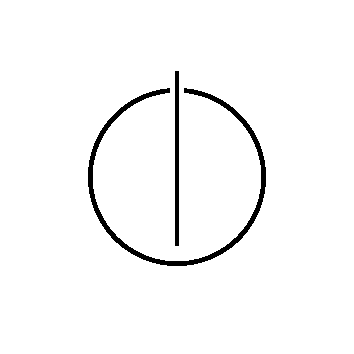
\includegraphics[width=4cm]{styles/informat.png}
  \end{figure}
   

\end{center}

% undo BCOR correction
\addtolength{\hoffset}{\bcorcor}

	
	
%	\input{components/cover_maschmeyer}
	\clearemptydoublepage
	
	% The titlepage for the CAMP report document.
% Included by MAIN.TEX


%--------------------------------------------------
% The title page
%--------------------------------------------------

% correct BCOR - undo at the end !!!
\def\bcorcor{0.15cm}
\addtolength{\hoffset}{\bcorcor}

\thispagestyle{empty}

 \vspace{10mm}
\begin{center}
	       \oTUM{4cm}
	   
	   \vspace{5mm}     
	   %\huge FAKULT{\"A}T F{\"U}R INFORMATIK\\ 
	   \huge DEPARTMENT OF INFORMATICS \\
	   \vspace{0.5cm}
	 %\large DER TECHNISCHEN UNIVERSIT{\"A}T M{\"U}NCHEN\\
	 \large TECHNISCHE UNIVERSIT{\"A}T M{\"U}NCHEN\\
        
	\end{center}
		

\vspace{10mm}
\begin{center}

   {\Large \doctype}

  \vspace{10mm}
  
  {\LARGE \title}\\
  
  
  \vspace{10mm}
  
  
  {\LARGE  \titleGer}\\
  
  
  \vspace{10mm}

    %\hfill
    \begin{tabular}{ll}
	   \Large Author:     & \Large \author \\[2mm]
	   \Large Supervisor:    & \Large Prof. Dr.-Ing. habil. Alois Knoll \\[2mm]
	   \Large Advisors:	& \Large Dr. Kai Huang\\ 
	                    & \Large Biao Hu, M.Sc.\\[2mm]
	   \Large Date:       & \Large April 15, 2015
	 \end{tabular}
	 
	 \vspace{5mm}
	 
	 \begin{figure}[h!]
  \centering
   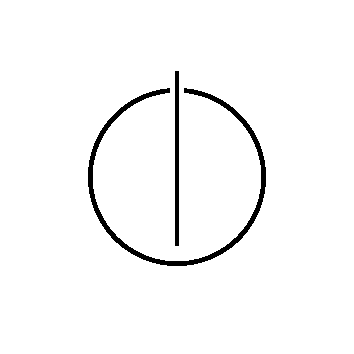
\includegraphics[width=4cm]{styles/informat.png}
  \end{figure}
   

\end{center}

% undo BCOR correction
\addtolength{\hoffset}{\bcorcor}

	
	
	\clearemptydoublepage


\thispagestyle{empty}
\selectlanguage{german}
	\vspace*{0.8\textheight}
	\noindent
	%Ich versichere, dass ich diese Diplomarbeit selbst{\"a}ndig verfasst und nur 
	%die angegebenen \\Quellen und Hilfsmittel verwendet habe.
	
	I confirm that this bachelor's thesis is my own work and I have documented all sources and material used.
	
	%TODO check space
	\vspace{15mm}
	\noindent
	M{\"u}nchen, \today \hspace{5cm} \author
\selectlanguage{english}
\newpage

	
	%\clearemptydoublepage
\phantomsection
\addcontentsline{toc}{chapter}{Acknowledgements}	


%\chapter*{Acknowledgements}

\vspace*{2cm}

\begin{center}
{\Large \bf Acknowledgments}
\end{center}

\vspace{1cm}




If someone contributed to the thesis... might be good to thank them here.
	
	% Abstract for the TUM report document
% Included by MAIN.TEX


\clearemptydoublepage
\phantomsection
\addcontentsline{toc}{chapter}{Abstract}





\vspace*{2cm}
\begin{center}
{\Large \bf Abstract}
\end{center}
\vspace{1cm}

%An abstracts abstracts the thesis!

Heterogeneous computing systems consisting of CPUs, GPUs and FPGAs currently suffer from a comparatively low bandwidth and high latency for data transfers between the GPU and the FPGA.
So far, no standard or vendor-provided method exists for direct communication between these two devices.
Indirect communication with a round-trip via the CPU is required.

This thesis enables this missing link over the PCIe bus for use with the popular high performance computing platform OpenCL.
%opencl
As expected, a significant increase in bandwidth has been achieved.
However, only the direction from the FPGA to the GPU could be realized.
More investigation or a different approach is still required to enable the opposite direction as well.





	\tableofcontents

%  \clearemptydoublepage

\phantomsection
\addcontentsline{toc}{chapter}{Outline of the Thesis}

\begin{center}
	\huge{Outline of the Thesis}
\end{center}




%--------------------------------------------------------------------
\section*{Part I: Introduction and Theory}

\noindent {\scshape Chapter 1: Introduction}  \vspace{1mm}

\noindent  This chapter presents an overview of the thesis and it purpose. Furthermore, it will discuss the sense of life in a very general approach.  \\

\noindent {\scshape Chapter 2: Theory}  \vspace{1mm}

\noindent  No thesis without theory.   \\

%--------------------------------------------------------------------
\section*{Part II: The Real Work}

\noindent {\scshape Chapter 3: Overview}  \vspace{1mm}

\noindent  This chapter presents the requirements for the process.
   \clearemptydoublepage

\phantomsection
\addcontentsline{toc}{chapter}{List of Abbreviations}

\begin{center}
	\huge{List of Abbreviations}
\end{center}


\vspace{3cm}


\begin{center}
\begin{tabular}{l p{12cm}}
	ATT & Address Translation Table in the Altera PCIe core\\
	BAR & PCI Base Address Register\\
	BSP & Board Support Package, IP stack for Altera OpenCL\\
	CPU & Central Processing Unit\\
	DDR & Double Data Rate, a type of memory\\
	DMA & Direct Memory Access\\
	DPU & Double-precision Floating Point Unit\\
	FIFO & First-In First-Out Queue\\
	FPGA & Field Programmable Gate Array\\
	GPGPU & General Purpose Computing on Graphics Processing Units\\
	GPU & Graphics Processing Unit\\
	HDL & Hardware Description Language\\
	HPC & High Performance Computing\\
	ICD & Installable Client Driver, library that acts as a proxy between different OpenCL implementations\\
	IOMMU & Input/Output Memory Management Unit\\
	IP  & Intellectual Property, usually refers to HDL code\\
	IPC & Inter-Process Communication\\
	LUT & Look-Up Table, refers to the basic FPGA building block\\
	MMIO & Memory Mapped Input/Output\\
	MMU & Memory Management Unit\\
	OpenCL & Open Computing Language, a popular HPC platform\\
	OS  & Operating System\\
	PCIe & Peripheral Component Interconnect Express Bus\\
	RAM & Random Access Memory\\
	RDMA & Remote Direct Memory Access\\
	SDK & Software Development Kit\\
	SMX & NVIDIA Streaming Multiprocessor\\
	
\end{tabular}
\end{center}


	\mainmatter
	
	
		% ---------------------------------------------------------------------------
		%
		%Introduction and Background Theory
		%
		% ---------------------------------------------------------------------------
		%\part[Introduction and Theory]{Introduction and Theory}
		%\label{part:introAndBackgroundTheory}
		\chapter{Introduction}


%%recent advances in machine learning
%% alphago, more examples. 
%TODO use alphago zero, it is stronger

Lee Sedol, one of the best Go players in the world, was beaten by the Go engine AlphaGo in a match. The engine was clearly stronger \cite{leesedol}.  
%TODO /cite{leesedol}
AlphaGo only knew the rules at the beginning and got stronger only by playing with itself. 
Artificial Intelligence is quite popular nowadays because of its many use cases: Self-Driving cars, playing atari games, robotics and more. 
But how do these engines learn how to get so good at their areas ? The answer is reinforcement learning, an area of machine learning. 

\vspace{0.5cm}

The idea of reinforcement learning is to have a state and actions that an agent can choose from. Each action results in different rewards and states. Rewards are used by agent to measure how good an action was. This process is repeated which results in the agent learning which actions in each state are better.
%TODO maybe find a better example with better reward
Imagine you are a soccer player. You are standing in front of the goal (which is the state you are in). You can either shoot or pass the ball (which are your available actions). You choose to shoot, but the ball is blocked by the goalkeeper (you got a low reward). So the next time you are in front of the goal again, you will more probably try to pass the ball. This time your teammate scored a goal (you got a high reward). From this experience you learn that it is probably better to pass the ball if you are standing in front of the goal.
The concept of reinforcement learning can be used in a variety of environments, for example robotic arms.

\vspace{0.5cm}

%%robotic arms uses

Already in the 14th century, Leonardo da Vinci made blueprints of robotic arms.
%TODO \cite{roboarmhistory} 

A robotic arm resembles a human arm. It consists of segments which are connected by joints. 
%TODO \cite{howroboarmworks}
The number of joints correspond to what is called Degrees of Freedom. A robotic arm with 5 joints would have 5 Degrees of Freedom because it can pivot in 5 ways. Each joint is connected to a step motor. Step motors make the robot move very precisely.
The equivalent to a human hand is the end effector. The end effector can vary depending on the tasks.  

\vspace{0.5cm}

Robotic arms have many advantages. They are very accurate and consistent which is why they are mostly used for repetitive tasks or tasks that require high accuracy which are hard for humans. 
%TODO \cite{roboarmuk} 
This is the main reason why they are used in laboratories and hospitals for surgeries. They can also be used automatically without any human which is why they are used for manufacturing and assembly lines. 

\vspace{0.5cm}

Humans still have to teach the robotic arms how to move when 
setting them up. For path planning of the robotic arm, a sequence of actions has to be found that solves the task. This sequence is saved and repetitively executed by the robotic arm. Finding the path still requires human labor. Either by testing or by using linear algebra a path can be found. 
%TODO find good cite 
A robotic arm needs 6 Degrees of Freedom to be able to move its end effector in every direction and orientation. This also means that robotic arms with more degrees of freedom do not have a unique path to solve the tasks. There are different paths which can vary in length and energy consumption.
To improve the quality of the path and to do path planning without a human, using reinforcement learning for robotic arms is a logical approach. 

\vspace{0.5cm}


%%reinforcement learning in robotics
%TODO cite papers with rl robotics
...

\vspace{0.5cm}

%%problems with reinforcement learning because of sparse rewards

There is an issue that prevents robotic arms to learn with reinforcement learning. It is hard to construct a suitable reward function for tasks where robotic arms are used. For example ... 
%TODO read HER paper, cite
So either a suitable reward function has to be constructed by hand, or the simplest reward function, a binary sparse reward function has to be used. 
Both approaches have some issues. 
Constructing a reward function can be quite complicated. Also, for each task an individual reward function has to be made. So someone has to do this work which defeats the purpose of using reinforcement learning for robotic arms over path planning by hand. Depending on the case it might be easier to just plan the path without reinforcement learning.
Using only a sparse reward for robotic arms is as follows. a reward is given, when the goal is reached, no reward is given when the goal is not reached. Robotic arms have usually many Degrees of Freedom, so there are many actions that can be taken by the robotic arm. It is quite unlikely for robotic arms to fulfill the task by doing random movements. Tasks like moving an object are near impossible to solve with random actions. 
%TODO Find prove-> at timestep 0 for fetchplace 
So it is very unlikely for the robotic arm to earn a reward and learn. It takes a very long time to train a robotic arm with sparse rewards.
But recently hindsight experience replay has been introduced. 
%TODO \cite HERPAPER]
Hindsight experience replay allows a high learning rate even with sparse rewards. 


\vspace{0.5cm}

%%her introduces

Hindsight experience replay works as follows.


\vspace{0.5cm}

%%many endeavors to use and improve her


%% some robotic arm tasks , eg. stacking stones
%%mostly work on improving her

\vspace{0.5cm}

%%using harder environments for her in this thesis to see if it also works.



This thesis is structured as follows: 
Chapter 2 describes the theoretical background on robotic arms, reinforcement learning and algorithms like deep deterministic policy gradients and hindsight experience replay. 
Chapter 3 explains the methodology used for this thesis.
Chapter 4 gives an overview of the simulation environment.
In chapter 5, the experiments are presented and the results are discussed.
In the last chapter, the results are summarized and suggestions for further work is provided.





		
		\chapter{Theoretical Background}

This chapter explains the concepts needed to understand this thesis. The theory behind RL, ANN, DDPG and HER is explained.

\section{Reinforcement Learning}
%% In context of machine learning (supervised,unsupervised)
%% potential to be better than humans

RL is one of the main learning concepts of Machine Learning next to Supervised Learning and Unsupervised Learning \cite{machinelearning}.
\newline
In Supervised Learning some input data is given to the learning agent. The agent is expected to come up with some output which is then compared with the expected output. If the output given by the agent and the expected output matches, then the agent was correct. The agent is trained by calculating the error between expected output and actual output. An use case for Supervised Learning is sorting mails into regular mail and spam mail. The agent is given a mail and it should decide whether the mail is regular or spam based on the content. Supervised Learning is used for classification and regression problems \cite{machinelearning}. It is mainly useful when the expected output is already known, so the learning agent can learn to do recognize these. 
\newline
In Unsupervised Learning there is no expected output. The learning agent is fed with data so it can figure out interesting features and similarities between different data. Unsupervised Learning is often used to cluster data, often pictures, based on similarities \cite{machinelearning}.
\newline
In RL the agent is learning through rewards that are given through interaction with an environment. The goal of a task is clear, but the path of actions to reach the goal is not trivial. RL is used to find the best action in each situation. It is often used for games because they are already set up to have a clear task and goal, but the optimal way to reach it is not clear. Games usually provide full information on the environment in contrast to the real world, therefore setting up the learning environment is simple. Also Supervised Learning is limited in performance because the agent can only learn to become as good the expected output that we set. So in games like chess, with Supervised Learning the agent can only become as good as the best players it learns from, but not better. It is limited by the skills of the best humans \cite{nolimit}. However, RL is not restricted by these limitations. The agent can improve on its own only by exploring his options. In games like Go and Chess, engines that use RL have already far surpassed the best human players \cite{alphazero}. 

\vspace{0.5cm}

%%general idea
This section will explain the theory behind RL. The post by Lilian Weng is recommended as a resource on more precise explanations on RL \cite{rllilianweng}. RL is usually modeled as a Markov Decision Process. The Markov Decision Process for RL consists of following elements \cite{rlwiki}:

\begin{itemize}
	\item A set of states S
	\item A set of actions A
	\item The transition probability $P_a(s,s')$ from state s to s' under action a
	\item The immediate reward $R_a(s,s')$ of that transition
	\item rules that describe the agents observation
\end{itemize}

The agent and environment are in a state s. The agent chooses an action a from its set of possible actions A to interact with the environment. The environment reacts by transitioning to another state and returning a reward R and an observation to the agent. Depending on the model the transitions might be stochastic or deterministic. The aim of the agent is to earn the maximal total reward possible. In order to reach this aim, the agent interacts with the environment to gain knowledge about the environment through the gained rewards and observations. Through this process, the agent learns in which state which actions are better to gain more reward. This is illustrated by Figure \ref{rl_general}.

\begin{figure} [h]
	
	\centering
	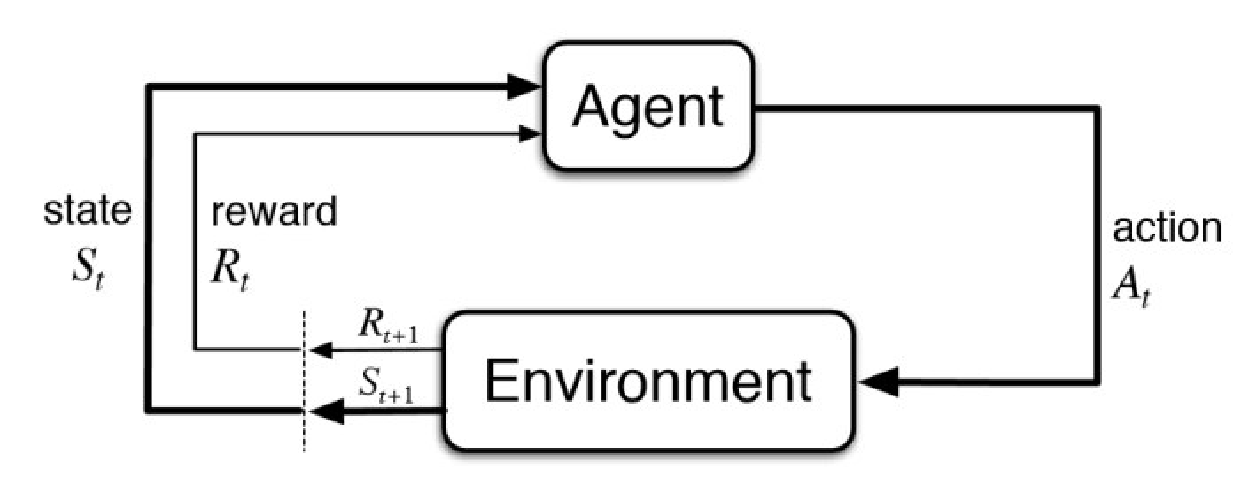
\includegraphics[width=1\textwidth]{figures/rl_general.pdf}
	\caption{Reinforcement Learning. An agent chooses an action to interact with the environment and gets a reward and an observation of his new state back. 
		\label{rl_general}	
		\cite{rl_general.jpg}
	}
\end{figure}

\vspace{0.5cm}

%policy 
In each state there is an action that the agent considers best due to its current knowledge about the expected rewards of each action. This set of actions is known as the policy 
$\pi (s)$. 
The goal of getting maximal reward can be interpreted as finding the best actions in each state that give the most reward, which is finding the optimal policy. The policy can also be either deterministic or stochastic, depending on the transition probability of the environment.

\vspace{0.5cm}

%value function
A value function is used to measure how good a state or action is. Two types of value functions are used for the states and the actions. the state value function is denoted as V(s). The value of a state is the expected reward when acting according to the policy 
$\pi$ \cite{rlwiki}.
V(s) is defined as follows in equation \ref{eq:state-value-function}.

\begin{equation}
\label{eq:state-value-function}
V^\pi (s) = \mathbb{E} [R | s,\pi]
\end{equation}

The actions value function is denoted as Q(s,a) and is defined In equation \ref{eq:action-value-function}.

\begin{equation}
\label{eq:action-value-function}
Q^\pi (s,a) = \mathbb{E} [R | s,a,\pi]
\end{equation}

When determining the value of a state or action, a discount factor $\gamma$
is used to discount future rewards towards immediate rewards. 
The idea is that a state s is not only as good as the reward you get when transitioning to that state. Future rewards from states that are reachable from state s should also be considered. The value of a state consists of the reward that you get by transitioning to that state and the potential rewards that can be gained by transitioning from that state. 
Since future rewards are not as certain as immediate rewards, the discount factor is used. The farther a reward is in the future, the more it is discounted. 
%bellman equations
The Bellman equations described in equation \ref{eq:V-bellman} and \ref{eq:Q-bellman} are a set of equations that convert the value functions into the immediate and future reward and can be used to update the value-functions \cite{rllilianweng}.

\begin{equation}
\label{eq:V-bellman}
V_\pi (s) = \sum_{a \in A}  \pi(a|s) (R(s,a) + \gamma \sum_{s' \in S} P_{ss'}^a V_\pi (s'))
\end{equation}

\begin{equation}
\label{eq:Q-bellman}
Q_\pi (s,a) = R(s,a) + \gamma \sum_{s' \in S} P_{ss'}^a \sum_{a \in A}  \pi(a'|s') Q_\pi(s',a')
\end{equation}

The goal is to find the actions that return the maximal reward. This is displayed by the Bellman optimality equations (\ref{eq:V-optbellman},\ref{eq:Q-optbellman}) \cite{rllilianweng}:

\begin{equation}
\label{eq:V-optbellman}
V_\ast (s) = \max_{a \in A} (R(s,a) + \gamma \sum_{s' \in S} P_{ss'}^a V_\ast (s'))
\end{equation}

\begin{equation}
\label{eq:Q-optbellman}
Q_\ast (s,a) = R(s,a) + \gamma \sum_{s' \in S} P_{ss'}^a \max_{a \in A} Q_\ast(s',a')
\end{equation}

To calculate the optimal values of each state and action, Dynamic Programming could be used if the entire model is known. But even knowing the entire model is not good enough as usually the main issue lies in the huge state and action space, which makes it impossible to use Dynamic Programming. For RL, artificial neural networks (ANNs) can be used to approximate the value functions \cite{neuralnetpath}. 

When following the current policy, the agent will earn the maximal reward that it could earn with current knowledge, but never more than that. To learn, the agent has to deviate from the policy and explore different actions and states. The question is how much deviation is necessary, as the agent also needs to exploit most of the policy path it has learned until now because following most of the policy has a higher probability of earning a high reward. This is known in RL as the exploration vs. exploitation problem. Usually there is a variable $\epsilon$ that determines with which probability the agent will deviate from the policy. It is set rather low to let the agent exploit most of its policy. As an example, an approach is $\epsilon$-greedy \cite{egreedy}. With a high probability of $1-\epsilon$ the agent will choose the policy and with a probability of $\epsilon$ a random action is chosen. This ensures that the agent exploits most of the policy, but also explores more possible actions that might bring more reward. 

%%neuronal networks
\section{Artificial Neural Networks}

ANNs are inspired by the human brain. 
%\nnbio, blablabla
The ANN consists of layers of neurons. Each neuron is connected to the next layer of neurons. There is one input layer and one output layer at the beginning and end of the layer of neurons. The layers between the input and output layers are called hidden layer. The hidden layer can consist of only one or more layers. The idea is to train the ANN to take inputs and produce outputs. To approximate the value functions the input would be states and actions, the output should be the correct and optimal values of these states and actions. An example of an ANN is shown in Figure \ref{neuralnet}.

\begin{figure} [h]
	\centering
	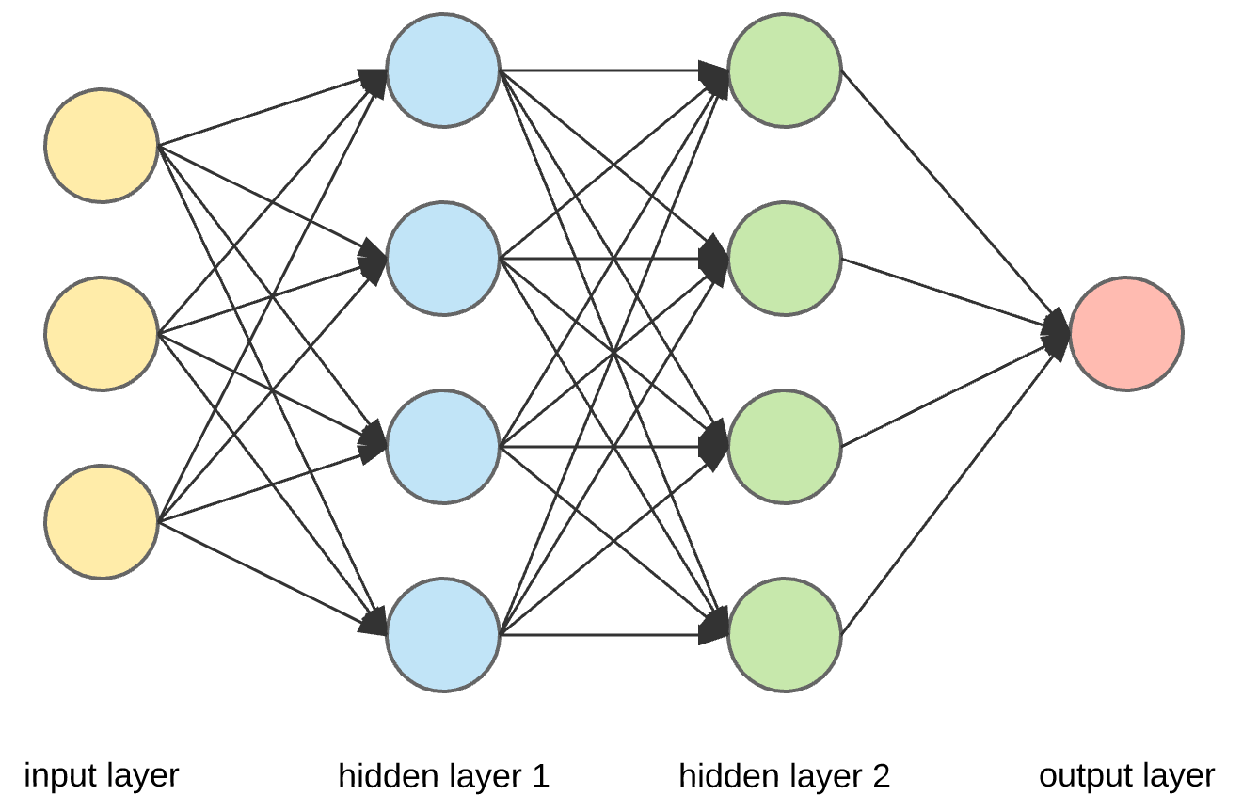
\includegraphics[width=1\textwidth]{figures/neural_network.pdf}
	\caption{A neural network. \cite{neural_networkpng}}
	\label{neuralnet}
\end{figure}

\vspace{0.5cm}

The learning process of the neuronal network is as follows. Each neuron obtains inputs $x_i$ by the the outputs of the neurons in the layer before it. Each input value is weighted and then the sum of these weighted values is taken. A bias $b$ is also added to support the learning process. After using an activation function on the sum, the value is output to the next layer of neurons. The activation function is a simple function that either reduces the output of the neuron to 0 if the value is below a certain threshold, otherwise the value is output unfiltered.
The training process of the neuron can be seen in Figure \ref{neuron}.
%besser formulieren!

\begin{figure} [h]	
	\centering
	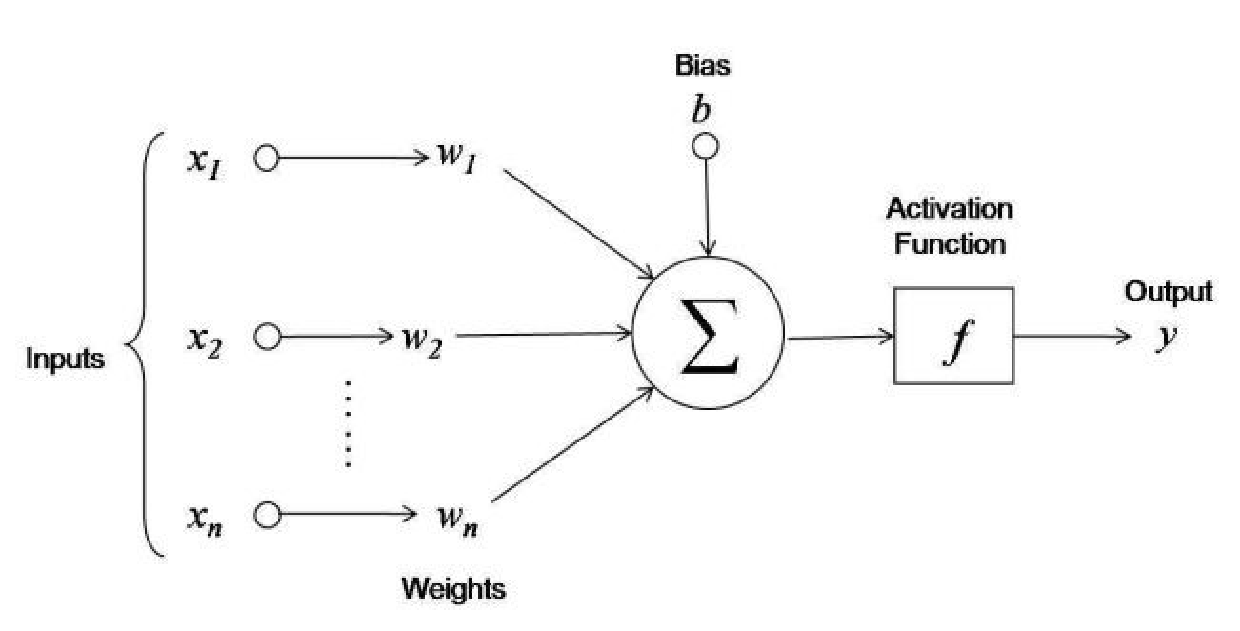
\includegraphics[width=1\textwidth]{figures/neuron.pdf}
	\caption{A neuron and how its value is composed \cite{neuron.jpeg}}
	\label{neuron}
\end{figure}

\vspace{0.5cm}

When the ANN outputs a value, a process called Backpropagation is used to improve the ANN \cite{backprop}. When initializing the ANN, the actual right weights for the input values are unknown, so random values for the weights are used. Therefore, the output values will not be right. By using an error function, the amount of error can be computed. The amount of error can be used to figure out how much the weights have to be modified for the output to become right. Backpropagation is the process of going backwards through the ANN and improving the weights of the neurons that caused the output value to be wrong. By repeating the whole process, the weight of each neuron converges towards an optimal value. 

\vspace{0.5cm}

\section{Deep Deterministic Policy Gradients}

The paper by Silver et al. is a recommended resource for more detailed explanations \cite{ddpg}. This chapter will give a short summary of DDPG.
The algorithm DDPG learns concurrently a Q-function (the action-value function) and a policy. \cite{ddpg}
Q*(s,a) is used to find the the optimal action in each state.
To compute the Q-values for a discrete action space, the Q-values of each action could be calculated and compared to find the biggest value. But in a continuous action space it is not possible to calculate the Q-value for each action. DDPG uses the fact that the action space is continuous and so Q*(s,a) is expected to be differentiable in respect to the action argument. \cite{ddpg}
This way it is possible to approximate the Q-values and policy.

\vspace{0.5cm}

To learn the Q-values, the Bellman equation for the action value is used. To approximate the Q-values, a mean squared Bellman error function is used.
The idea is that minimizing this function error is equal to approximating the current Q-values to the optimal Q-values.

\vspace{0.5cm}

For DDPG an experience replay buffer is also used. The replay buffer is a set of experiences. This can be used to replay old experiences. When only using new experiences, the ANN might be overfit to those experiences. Being overfit means that for some experiences the ANN will output very good results, but for most other experiences it will perform very bad. Experience replay is useful to prevent that. But a too large buffer can cause the learning process to slow down. The right balance has to be found.

DDPG also uses target networks. Equation \ref{eq:target} is called target \cite{ddpg}.

\begin{equation}
\label{eq:target}
r + \gamma (1-d) \max_{a'} Q_\phi(s',a')
\end{equation}

The target is what is desired for the Q-function to approximate to.
When minimizing the mean squared bellman error function, there is the problem that the target is also dependent on the parameters that are trained. When changing the parameters, the target would also change which is problematic. That is why the target network, a copy of the ANN is used. The update of the target network is delayed to avoid this conflict.
To find the optimal policy, simply gradient ascent can be used to find the maximal Q-values.


\section{Hindsight Experience Replay}

%subsection curriculum learning ?

%read paper, use it
Sparse rewards are a big issue in RL, especially in tasks for robotic arms often the rewards are sparse. Having sparse rewards means that most of the samples used for training will not successful and therefore will not bring any useful reward. For example, the task to move an object to a certain point would have a sparse reward for a robotic arm because very precise movements are needed which the robotic arm has to learn first.
 
\vspace{0.5cm}
 
Andrychowicz et al. have shown that HER can be used to deal with this issue for robotic arms \cite{herpaper}
HER can learn efficiently from sparse rewards and can also be combined with any off-policy RL algorithm.
This technique is inspired by the ability of humans to learn from failures as least as much as from successes.

\vspace{0.5cm}

HER works as follows. After an episode of gaining experiences, all transitions between the states in each training sample is stored in a replay buffer, but the goal that was not achieved is extended to a set with a goal that is reached. This can also be further extended to a set of more goals that can be achieved in the terminating state of the training sample. If the goal was to move an object to point x, but it was pushed to point y, the replay buffer would use the same transitions but change the the goal we wanted to achieve to y. So when replaying the same experience, the agent would be successful and earn an useful reward. This does not help the agent learn how to reach the goal it wanted to reach initially, but it learns how to reach other goals. Being able to reach those other already achieved goals might be beneficial in learning how to reach the goal it actually wanted to achieve. HER is mainly used for tasks with multiple goals, but it was shown that it also improves the training of tasks with only a single goal. \cite{herpaper}
Interestingly, Andrychowicz et al. have shown HER performs has problems when using shaped rewards. \cite{herpaper}
%add binary rewards at start of section ?. binary != shaped ?
 
 %add pseudocode ?

		
		
\chapter{Implementation of an Installable Client Driver for Altera OpenCL}
\label{section:icd}

As of SDK version 13.1 (which is used in this thesis) all Altera OpenCL functions are implemented in the dynamic library \texttt{libalteracl.so}.
Using this library directly inhibits the use of a second OpenCL implementation from a different vendor in the same application.
Trying to link both libraries during compilation will fail due to conflicting multiple symbol definitions.

The \texttt{cl\_khr\_icd} OpenCL extension \cite{icd} defines the \emph{Installable Client Driver} (ICD) and the \emph{ICD Loader} libraries that act as a proxy between the user program and the actual implementations.
With this extension, the vendor implementations are loaded at run time, avoiding the issue of symbol conflicts.
The application is then linked to the ICD Loader instead of the individual vendor libraries.
Figure \ref{fig:icd} illustrates the relationships between the libraries.
Currently, Altera does not provide an ICD for its SDK.
A minimal ICD was implemented during this thesis and it is documented in this section.


%NVIDIA ICD is called libnvidia-opencl.so.1 and dlopens (most likely) libcuda.so
\begin{figure}[htb]
\centerline{
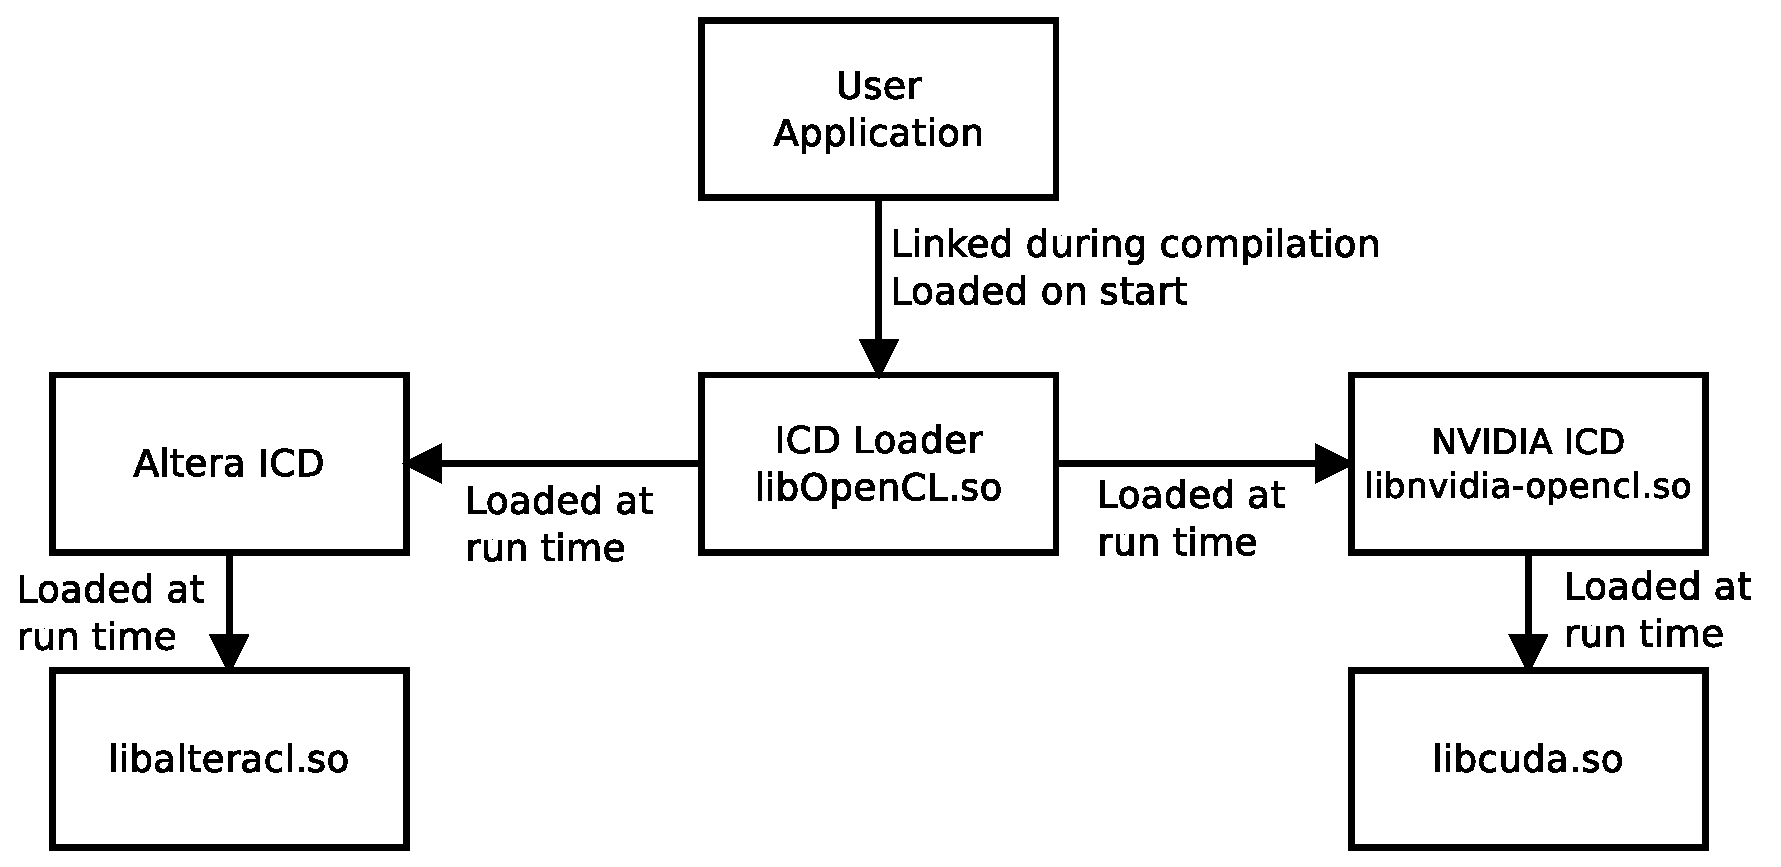
\includegraphics[width=0.85\textwidth]{images/icd.eps}}
\caption{Relationship between the dynamic libraries}
\label{fig:icd}
\end{figure}


%extension specs

To enumerate vendor ICDs on Linux, the ICD Loader scans the files located in the path \texttt{/etc/OpenCL/vendors} \cite{icd}.
These files have to contain a single line with the absolute or relative path to the actual vendor ICD dynamic library.
The loader will then attempt to load this library using \texttt{dlopen}.
%If successful, the functions \texttt{clIcdGetPlatformIDsKHR}, \texttt{clGetPlatformInfo}, and \texttt{clGetExtensionFunctionAddress} are queried.

The extension re-defines all OpenCL functions and objects.
When the user application calls an OpenCL function it actually calls one of those re-defined functions from the ICD Loader.
The first function, of an OpenCL application is usually \texttt{clGetPlatformIDs}.
When it is called, the ICD Loader iterates over all known vendor ICDs and in turn calls their \texttt{clGetPlatformIDs}.
The vendor ICD then returns a pointer to a struct which has to contain the new \texttt{KHRicdVendorDispatch} struct, as in listing \ref{listing:structplatform}.

\begin{lstlisting}[label=listing:structplatform, caption=Definition of \texttt{struct \_cl\_platform\_id} in the Altera ICD, morekeywords={}]
struct _cl_platform_id
{
    KHRicdVendorDispatch *dispatch;
    cl_platform_id actual_altera_platform_id;
};
\end{lstlisting}


%The extension redefines all OpenCL functions and objects. The objects have to contain the \texttt{KHRicdVendorDispatch} struct, as in listing \ref{listing:structqueue} using the example of \texttt{cl\_command\_queue}.

%\begin{lstlisting}[label=listing:structqueue, caption=Definition of \texttt{struct \_cl\_command\_queue} in the ICD Loader \cite{icd,icdloadersrc}, morekeywords={}]
%struct _cl_command_queue
%{
%    KHRicdVendorDispatch *dispatch;
%    // ... remainder of vendor-defined internal data
%    // e.g the actual cl_command_queue
%};
%\end{lstlisting}

All other OpenCL objects have to contain the \texttt{KHRicdVendorDispatch} struct too.
The \texttt{KHRicdVendorDispatch} contains a list of pointers to all remaining vendor ICD wrapper functions.
The vendor ICD has to fill in this struct.
When the user application calls another OpenCL function, the ICD Loader calls the appropriate function pointer from the dispatch struct.
This way the correct vendor is automatically inferred.
For clarification, the implementation of the \texttt{clFinish} function inside the ICD Loader is shown in listing \ref{listing:clFinish}.
\begin{lstlisting}[label=listing:clFinish, caption=Implementation of \texttt{clFinish} in the ICD Loader \cite{icdloadersrc}, morekeywords={dispatch}]
clFinish(cl_command_queue command_queue)
{
    return command_queue->dispatch->clFinish(command_queue);
}
\end{lstlisting}

The wrapper function in the vendor ICD has then to call the actual OpenCL function and pass it the real object, i.e. without the dispatch struct.
Unfortunately this cannot be automated because of functions which accept more than one OpenCL object or those that create new objects.
Every OpenCL function has to be re-implemented again manually.
The listing \ref{listing:clFinishIMPL} shows how this can be realized, using again the example of \texttt{clFinish}.
Here, \texttt{private\_dispatch} is another internally used dispatch which stores the real Altera function pointers.
The diagram in figure \ref{fig:icd2} illustrates the complete procedure.





\begin{lstlisting}[label=listing:clFinishIMPL, caption=Implementation of the wrapper function \texttt{\_icd\_clFinish} in the Altera ICD, morekeywords={}]
cl_int CL_API_CALL
_icd_clFinish(cl_command_queue   command_queue)
{
	cl_command_queue 
	real_queue  = ((struct _cl_command_queue*)command_queue)->queue;
	return( private_dispatch.clFinish( real_queue ) );
}
\end{lstlisting}


%TODO: maybe notes to the arrows: linked at compiletime, function pointer from dispatch, loaded dynamically
\begin{figure}[htb]
\centerline{
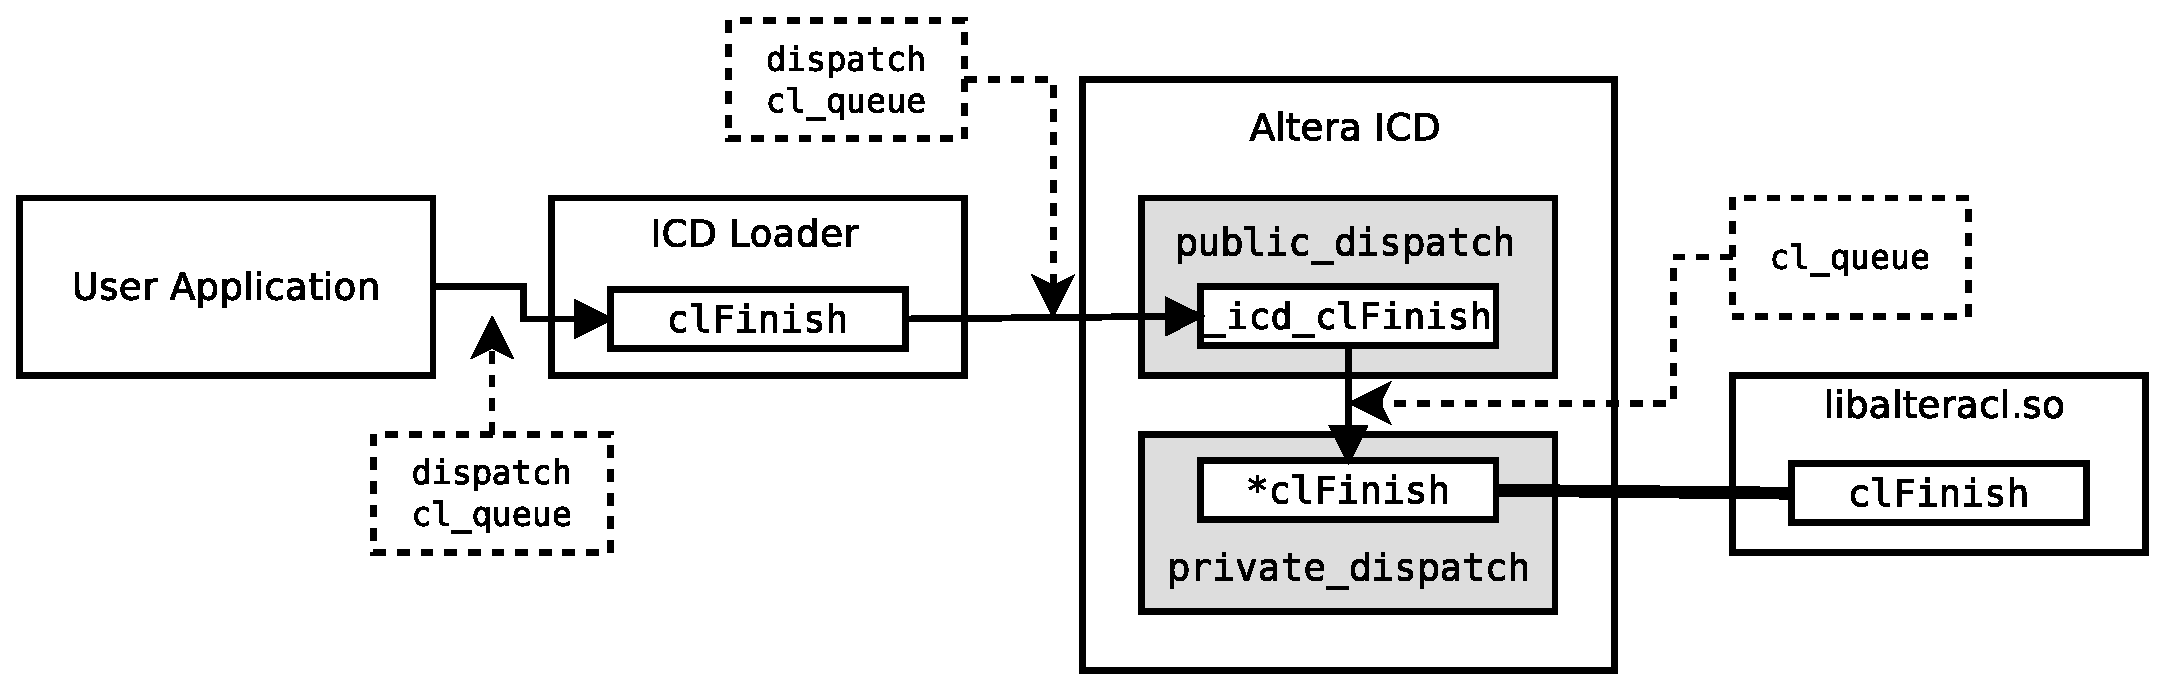
\includegraphics[width=1.1\textwidth]{images/icd3.eps}}
\caption{Call graph for the function \texttt{clFinish}.
The application calls the ICD loader function, which forwards the call to the wrapper function in the vendor ICD stored in the dispatch struct.
The wrapper function then calls the real OpenCL function.
The dashed boxes illustrate the contents of the arguments.}
\label{fig:icd2}
\end{figure}




%actual implementation
%The ICD loader opens the individual ICD libraries with the \texttt{dlopen} function \emph{without} the \texttt{RTLD\_DEEPBIND} flag \cite{icdloadersrc}.

The Altera ICD cannot be linked to the main library \texttt{libalteracl.so} which defines the actual OpenCL functions during compile time. This would again result in symbol conflicts, this time with the ICD Loader.
Instead, it must be loaded with \texttt{dlopen} during the run time.
\texttt{libalteracl.so} depends on \texttt{libelf.so}, \texttt{libalterammdpcie.so} and \texttt{libalterahalmmd.so}, which means these libraries have to be loaded beforehand with the \texttt{RTLD\_GLOBAL} flag.
This flag allows subsequently loaded libraries to use the symbols defined in the library to be loaded \cite{dlopen}.
While the \texttt{libelf.so} can be loaded without problems, the other two libraries in turn depend on \texttt{libalteracl.so} itself, creating a circular dependency.
A solution to this problem is to open \texttt{libalteracl.so} first with the \texttt{RTLD\_LAZY} flag and afterwards the other libraries with the opposite flag \texttt{RTLD\_NOW}.
With \texttt{RTLD\_LAZY}, a lazy binding is performed, that means the symbols are only resolved when needed, whereas \texttt{RTLD\_NOW} resolves all symbols before \texttt{dlopen} returns \cite{dlopen}.


Moreover to avoid conflicts with already loaded OpenCL symbols (defined by the ICD loader itself), the flag \texttt{RTLD\_DEEPBIND} is required.
This flag specifies that the library to be loaded should use its own symbols in preference to already loaded global symbols with the same name \cite{dlopen}.
The correct sequence of \texttt{dlopen} operations and flags is shown in listing \ref{listing:dlopen}.

\begin{lstlisting}[label=listing:dlopen, caption=Dynamically loading Altera OpenCL libraries, morekeywords={}]
dlopen( "libelf.so", RTLD_NOW | RTLD_GLOBAL | RTLD_DEEPBIND );
dlopen( "libalteracl.so", RTLD_LAZY | RTLD_GLOBAL | RTLD_DEEPBIND );
dlopen( "libalterammdpcie.so", RTLD_NOW | RTLD_GLOBAL | RTLD_DEEPBIND );
dlopen( "libalterahalmmd.so", RTLD_NOW | RTLD_GLOBAL | RTLD_DEEPBIND );
\end{lstlisting}


Loading the actual functions is accomplished with the \texttt{dlsym} function as in listing \ref{listing:dlsym}.
They will be stored in a second dispatch struct, only for use within the ICD.


\begin{lstlisting}[label=listing:dlsym, caption=Dynamically loading the original \texttt{clFinish} and filling in the dispatch, morekeywords={}]
private_dispatch.clFinish 
   = (KHRpfn_clFinish)dlsym(libalteracl_handle, "clFinish");
errmsg=dlerror();
if(errmsg!=NULL){return(-1);}
public_dispatch.clFinish=&_icd_clFinish;
\end{lstlisting}





The OpenCL specification defines more than 100 functions, most of them are very rarely used.
Therefore only the following most common OpenCL functions have been wrapped for this thesis:
\begin{center}
\begin{tabular}{ l  l  l}
	\texttt{clGetPlatformIDs} & \texttt{clGetPlatformInfo} & \texttt{clGetDeviceIDs}\\
	\texttt{clGetDeviceInfo}& \texttt{clCreateCommandQueue} & \texttt{clCreateContext} \\
	\texttt{clCreateBuffer} &   \texttt{clCreateProgramWithBinary} & \texttt{clBuildProgram}\\
	\texttt{clCreateKernel} & \texttt{clEnqueueNDRangeKernel} &   \texttt{clSetKernelArg}\\
	\texttt{clEnqueueReadBuffer} &   \texttt{clEnqueueWriteBuffer} & \texttt{clFinish}\\
\end{tabular}
\end{center}

Trying to call a function not in this list will result in a segmentation fault.
Moreover, none of the \texttt{clEnqueue*} functions listed above support OpenCL \emph{events}.
Events can be sometimes useful for asynchronous operations, i.e. those that do not block.
To support events, a complex memory management system that tracks the lifetime of the event objects is required.%, which goes beyond the scope of this thesis.


Though incomplete, this set of functions allows a fully functional OpenCL application to be built and used together with implementations from other vendors within the same process.
Additional functions can be added, as described above.


		
		\chapter{Implementation of Direct GPU-FPGA Communication}
\label{section:implementation}

%GPUDirect RDMA method will be used
In this thesis, a similar approach as described by Susanto \cite{susanto} will be used for the direct GPU-FPGA communication.
The transfer will be handled mainly by the DMA controller on the FPGA.
The CPU will only coordinate the transfer.
On the GPU side the NVIDIA GPUDirect RDMA mechanism is required.


%TODO:
%RDMA theory?
%dataflow inside the fpga, avalon etc
%implementation of the cpu-fpga dma
%kernel-to-user interrupts for dma
%basic rdma implementation only one descriptor at a time
%advanced: merge descriptors, bursts?


\section{Altera PCIe Driver and IP Overview}

%dma controller: dma-write/dma-read
%msgdma diagram
%hard pcie ip, ATT
%cpu-fpga dma?


%TODO: dma descriptor

Altera's OpenCL implementation consists mainly of a dynamic Linux library, a PCIe driver and a \emph{Board Support Package} (BSP) containing the Intellectual Property (IP) cores to be deployed on the FPGA \cite{altera_driver}.
The dynamic library is proprietary but the BSP and the driver are open source and can be analyzed and modified.

The components of the Altera OpenCL IP stack are interconnected by the \emph{Avalon Memory-Mapped} (Avalon-MM) interconnect \cite{altera_driver, avalon}.
Avalon-MM is a multi-master/multi-slave bus.
An address range is assigned to each slave connected to the bus.
The master can then initiate transactions to specific slaves by writing to or reading from the corresponding slave addresses, similarly to memory-mapped I/O on the Linux operating system.

The most important cores for this thesis are the PCIe core, the DMA controller core and the DDR memory interface.
Figure \ref{fig:avalonstack} provides an overview of the connections between them.
When the driver writes to the FPGA's PCIe BAR with some additional offset, the PCIe core forwards the data from its RX port to the Avalon interconnect.
Depending on the offset the message is routed to one of the slaves.
In this specific example, to communicate with the DMA controller, the driver has to write to the address \texttt{0xc800} within the FPGA BAR.

\begin{figure}[htb]
	  \centerline{
		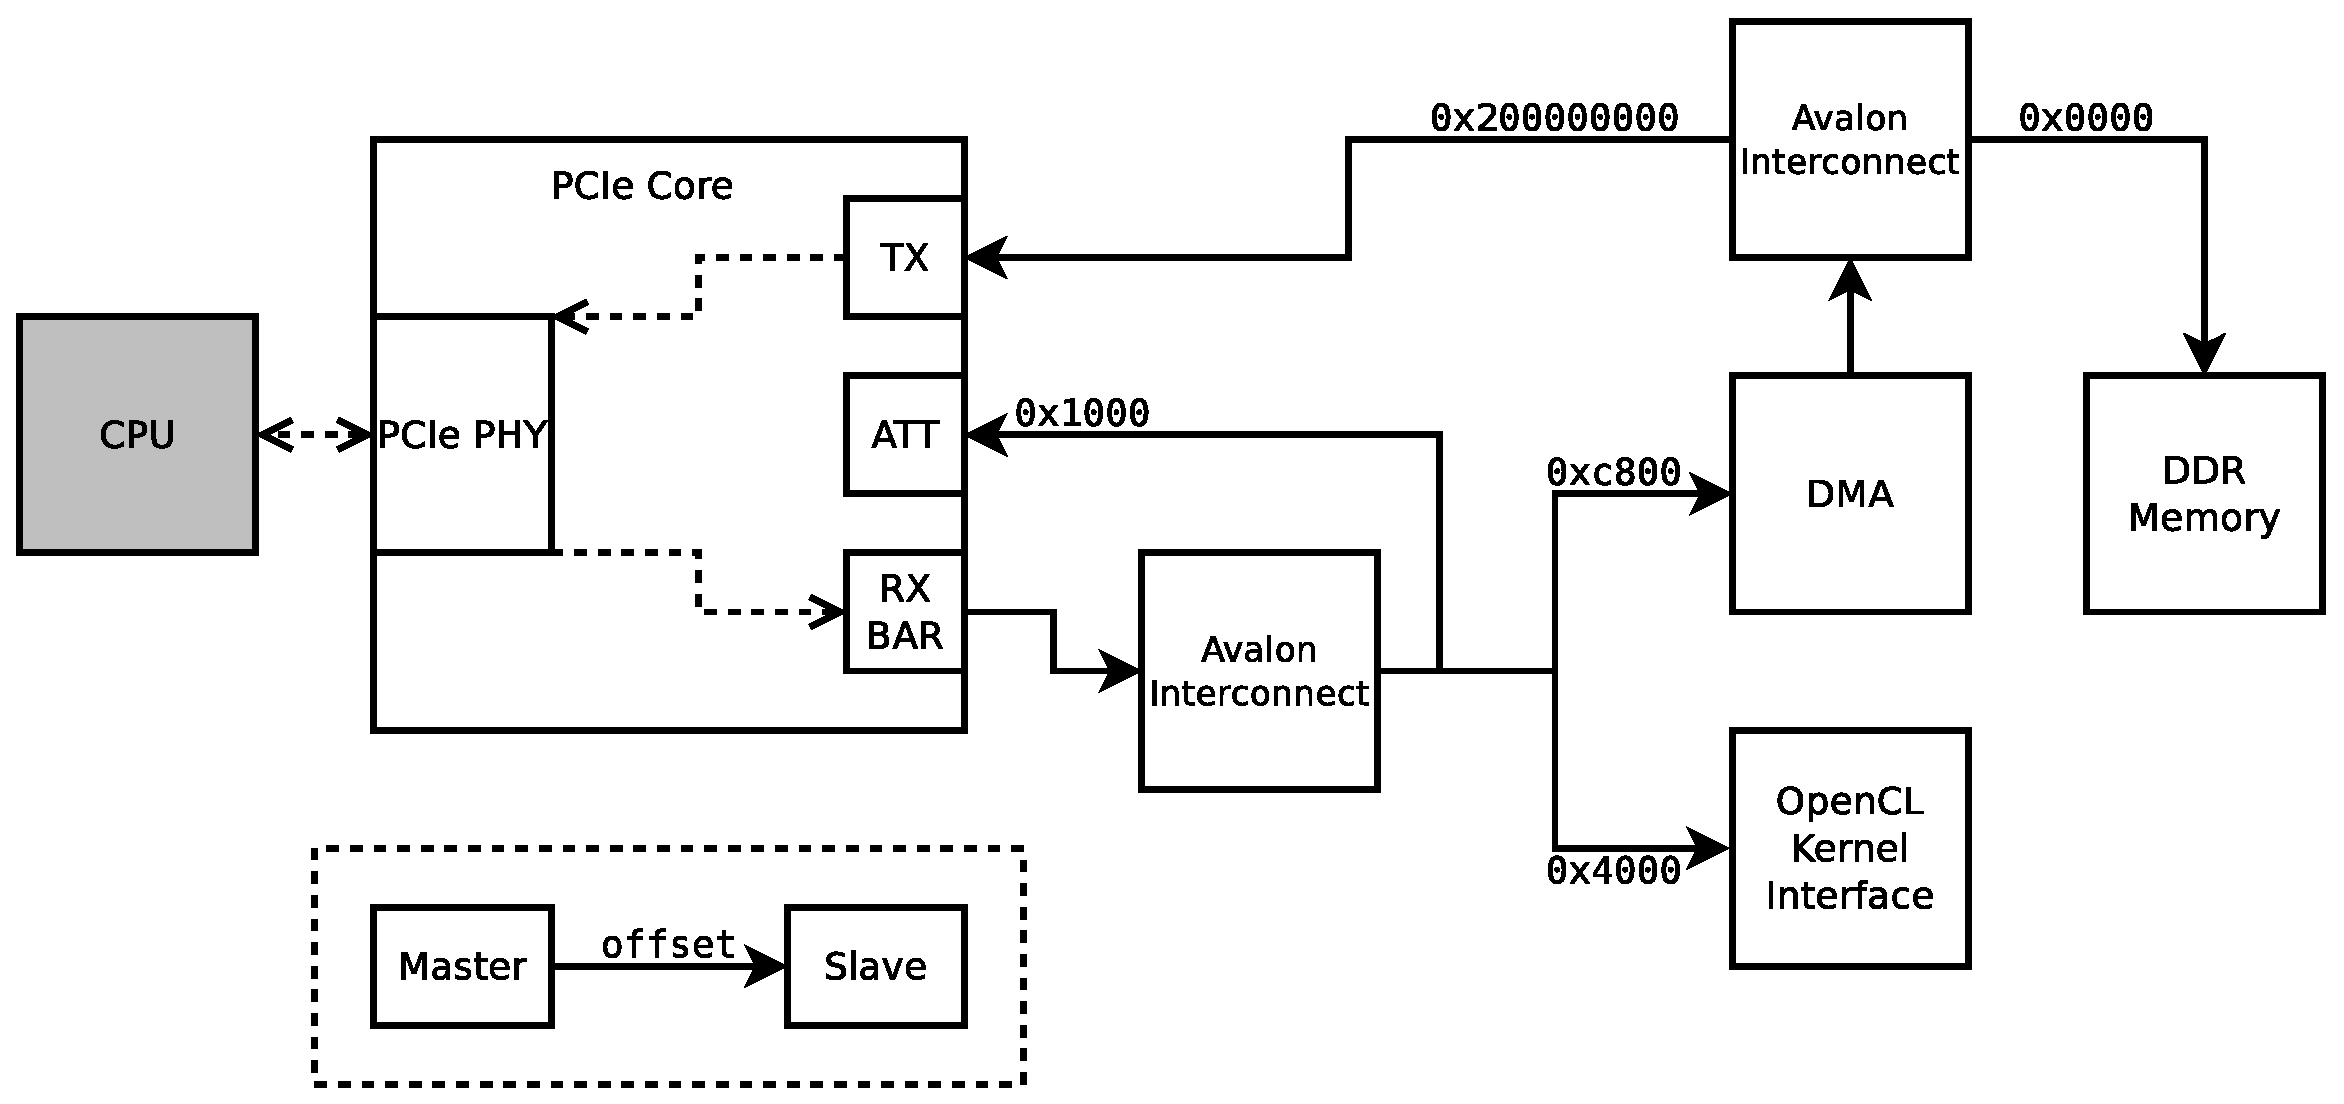
\includegraphics[width=1.1\textwidth]{images/avalonstack2.eps}}
	  \caption{Simplified configuration of the Altera  OpenCL IP stack on the FPGA.
	           Note that the solid arrows represent master/slave relationships and not necessarily the data flow direction.}
	  \label{fig:avalonstack}
\end{figure}


The DMA controller is a \emph{Modular Scatter-Gather DMA} (mSGDMA) IP core \cite{altera_msgdma}.
It is subdivided into a read master, write master and a dispatcher which coordinates the other two components.
A transfer is initiated by writing a 32-byte \emph{descriptor} to the dispatcher.
The descriptor contains all the required information about the desired transfer, including the source and destination memory addresses and the number of bytes to be transmitted.
Then, the dispatcher pushes the descriptors into a FIFO and processes them sequentially.

%descriptor fifo
%control parameter



The PCIe core contains an \emph{Address Translation Table} (ATT) which stores physical PCIe addresses \cite{altera_pcie_core}.
With an ATT, the DMA controller does not need to differentiate between physical addresses or addresses pointing to on-board DDR memory.
Instead, it can simply write the address it received in the descriptor from the device driver to the Avalon master port.
The Avalon interconnect will then route the signals to either the PCIe core or the FPGA memory.
The PCIe core would then select the required physical address from the ATT.
The differentiation has to made by the device driver.
To specify a physical address it has first to store it in the ATT by writing to offset \texttt{0x1000} (plus the ATT row number).
Then it writes to the offset \texttt{0xc800} (the DMA Controller) the address of the PCIe TX port as seen from the DMA. i.e. an offset of \texttt{0x200000000} plus the ATT row number.
Listing \ref{listing:rdma_pcietxs} shows this calculation in a more portable manner with the macros already defined in the Altera PCIe driver code.
%Then it calculates the address as in listing \ref{listing:rdma_pcietxs} and sends it to the DMA controller.



\begin{lstlisting}[label=listing:rdma_pcietxs, caption=Calculation of the PCIe address as seen from the DMA controller]
unsigned long
pcietxs_addr = (size_t)     ACL_PCIE_TX_PORT 
                 | (att_row *   ACL_PCIE_DMA_MAX_ATT_PAGE_SIZE) 
                 | (physical_addr  &  (ACL_PCIE_DMA_MAX_ATT_PAGE_SIZE - 1));
\end{lstlisting}


The direction of the transfer, i.e. whether data is to be read from or written into the FPGA memory, is specified implicitly by the \texttt{read\_address} and \texttt{write\_address} fields of the descriptor similar to listing \ref{listing:rdma_direction}.

\begin{lstlisting}[label=listing:rdma_direction, caption=Selection of the transfer direction ]
if(direction == READING)
{
	//reading from FPGA memory to PCIe bus
	dmadescriptor.read_address     = fpga_address;
	dmadescriptor.write_address    = pcietxs_address;
}
else
{
	//writing to FPGA memory from PCIe bus
	dmadescriptor.read_address     = pcietxs_address;
	dmadescriptor.write_address    = fpga_address;
}
\end{lstlisting}



\section{GPUDirect RDMA Overview}
\label{section:rdmaoverview}

NVIDIA GPUDirect \cite{gpudirect} is a family of technologies for fast data transfers in high performance computing systems with multiple devices.
Its key features include  an accelerated pipeline for video capture devices, storage devices, peer to peer memory access between GPUs and RDMA (Remote Direct Memory Access).
RDMA, as the name implies, is mainly intended to transfer data over network to or from other nodes in a compute cluster.
However it can also be used to transfer data to other third party PCIe devices within the same root complex.
One limitation is that it can only be used for NVIDIA Quadro and Tesla graphics cards.
Furthermore, systems which employ an IOMMU are not compatible.


The main idea behind GPUDirect RDMA is that the GPU can expose a region of its global memory into a PCIe BAR \cite{rdma}.
This can then be used by third party devices to access the memory region directly without the round-trip via the CPU.

Since version 4.0, the CUDA platform, on which NVIDIA's OpenCL implementation is based, uses a memory address management system called \emph{Unified Virtual Addressing} (UVA) \cite{cudaguide, rdma}.
With UVA the GPU memory pages are mapped into the system's virtual address space providing a single address space instead of multiple address spaces, one for the CPU and one for each GPU.
For the CUDA platform this simplifies the programming interface, but on the other hand requires pinning for DMA transfers. 


The NVIDIA device driver provides the function \texttt{nvidia\_p2p\_get\_pages} to pin a GPU memory region \cite{rdma}.
This function must be called from within the kernel space, i.e. from the third party device driver.
It accepts a virtual GPU address and, if the pinning is successful, returns a page table struct containing the physical addresses to each GPU memory page.
The virtual GPU address must be aligned to a 64KB boundary.
The listing \ref{listing:rdma_pinning} provides an example of this process.
\texttt{nvidia\_p2p\_put\_pages} is the corresponding function to unpin the pages.
Additionally, a callback function has to be registered which has to call the function \texttt{nvidia\_p2p\_free\_page\_table} to release resources.
This callback is invoked by the NVIDIA driver when it has to revoke the mapping for some reason.
This is mostly the case when the associated user process terminates.


\begin{lstlisting}[label=listing:rdma_pinning, caption=Pinning GPU memory \cite{rdma}, morekeywords={nvidia_p2p_get_pages}]
// do proper alignment, as required by NVIDIA kernel driver 
u64 virt_start = ((u64)address) & GPU_BOUND_MASK;
u64 pin_size   = ((u64)address) + size - virt_start;

struct nvidia_p2p_page_table page_table;
nvidia_p2p_get_pages( 0, 0, virt_start, pin_size, 
                             &page_table, free_callback, &page_table ); 
\end{lstlisting}

For Kepler class GPUs the pages typically have a size of 64KB.
The PCIe BAR is up to 256MB large of which 32MB are reserved for internal use.
This means that, in theory, up to 224MB can be pinned at a time \cite{rdma}.
However, during development, this number has been found to be slightly smaller, around 200MB.

\section{Extension of the Altera PCIe Driver}

%TODO: how does the OpenCL lib interact with the driver?
%separated RDMA and original DMA

The DMA component of the PCIe device driver provided by Altera expects a virtual address that maps to the CPU memory.
It tries to pin the buffer with the \texttt{get\_user\_pages} function to get a list of the pages and their physical addresses.
Simply passing a GPU address to the module will thus result in an error.
Neither will it work by just replacing \texttt{get\_user\_pages} with  \texttt{nvidia\_p2p\_get\_pages}, the corresponding GPU memory pinning function, due to assumptions related to the address space (for example about the page size) and differences in the pinning work flow.
A new RDMA component, managing only the direct GPU-FPGA communication, will thus extend the driver.
Transfers to and from CPU memory will be handled by the original code which shall remain untouched as far as possible.

%
New driver commands \texttt{ACLPCI\_CMD\_RDMA} and \texttt{ACLPCI\_CMD\_RDMA\_UPDATE} are added to differentiate between the original DMA and the new RDMA transfers.
They are issued via file I/O to the \texttt{/dev/acl0} device file, the same way as the original commands.
%TODO? \texttt{aclpci\_rw}
Section \ref{section:userspace} describes in detail how to use the new commands from user space.



\subsection{Basic Version}
%interrupts override
%new commands

%caveats: have to update the original aclpci struct to not confuse the original dma module
%e.g. dma_data.m_old_done_count inside the interrupt handler


%describe why basic version first

To avoid unnecessary complications during development only a very basic RDMA mechanism has been implemented first.
Its limitations include:
\begin{itemize}
	
\item Only one active transfer at a time
\item Only one active descriptor at a time. The next descriptor is sent only after the previous one is finished.
\item The size of descriptors fixed to 4KB. This is equivalent to the maximum size of an ATT entry.
\item Overall transfer size limited to 192MB. As noted in section \ref{section:rdmaoverview} this is roughly the maximum that can be pinned at a time.
\end{itemize}
Section \ref{sec:optimizations} provides an overview over some improvements to this version.

The new RDMA component consists of five main functions. Figure \ref{fig:driver_functions} illustrates their relationship. Their semantics are as follows:


\begin{figure}[htb]
	  \centerline{
		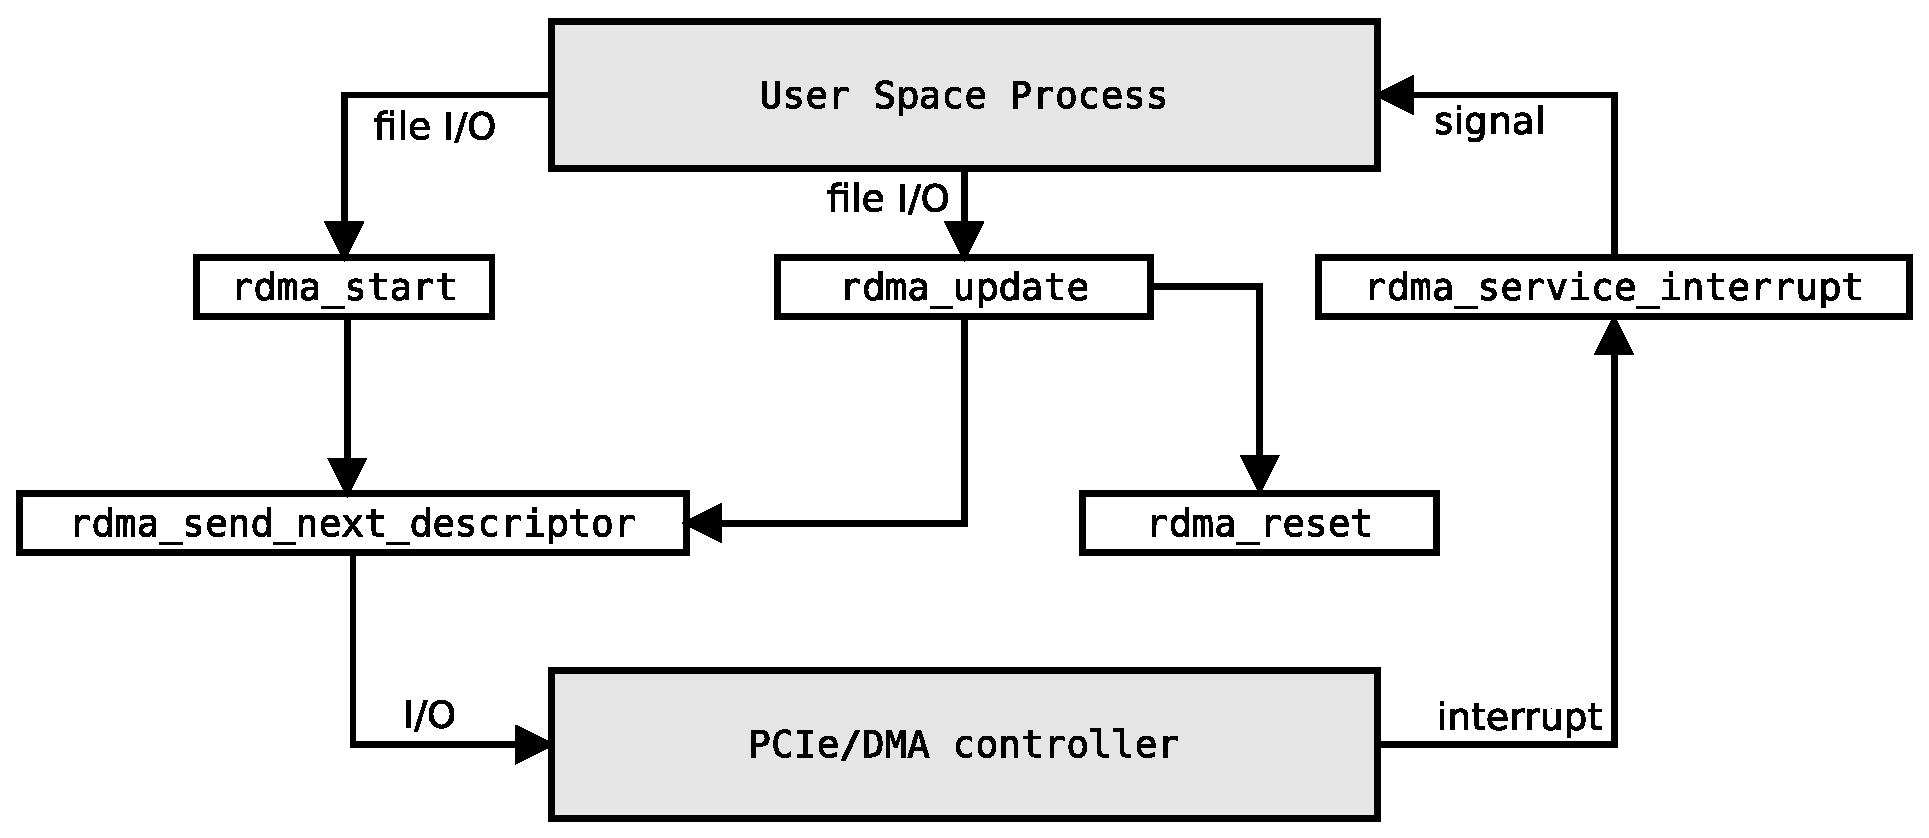
\includegraphics[width=1.0\textwidth]{images/driver_functions.eps}}
	  \caption{The main functions of the new RDMA component}
	  \label{fig:driver_functions}
\end{figure}



%TODO? no state stored between transfers? transfers independent of each other

\begin{list}{$\triangleright$}{\leftmargin=1.0em \itemindent=0em}
%\begin{itemize}
	\item {\bf \texttt{rdma\_start}}: The entry point for all RDMA transfers, invoked when the user space program issues the new \texttt{ACLPCI\_CMD\_RDMA} driver command.
	If there is no other active RDMA transfer, it tries to pin the supplied virtual GPU address as in listing \ref{listing:rdma_pinning}.
	If successful, the actual transfer is started by calling the \texttt{rdma\_send\_next\_descriptor} function.
	
	%TODO: not just  'tries to pin', calls kmd_pin...(), und diese funktion in listing
	%TODO: außerdem diagram updaten
	
	
	\item {\bf \texttt{rdma\_send\_next\_descriptor}}:
	This function performs the actual communication with the DMA controller on the FPGA.
	%TODO: %FIXME: It sets one ATT entry, sets up the dma descriptor
	%TODO: ... as described in section altera pcie overview
	It has to write the physical GPU address to an ATT entry of the PCI core and send a descriptor with the addresses and the size of the transfer.
	After this function, the driver terminates the execution and returns the control to the user space.
	



	
	
	\item {\bf \texttt{rdma\_update}}: This function is invoked from user space with the new driver command \texttt{ACLPCI\_CMD\_RDMA\_UPDATE} to continue with the transfer.
	If the previous descriptor has finished, it calls \texttt{rdma\_send\_next\_descriptor} to send the next one.
	It returns \texttt{1} if there is still data remaining to be transferred and \texttt{0} when the transfer finished to inform the user program.
	%TODO
	
	
	
	\item {\bf \texttt{rdma\_service\_interrupt}}: This is the new DMA interrupt handler for the device driver.
	It replaces the previous interrupt handler \texttt{aclpci\_dma\_service\_interrupt} from the original DMA code.
	It is called whenever the DMA controller signals an interrupt, i.e. when a descriptor is finished.
	Its first task is to acknowledge the interrupt by clearing the IRQ bit as soon as possible, to avoid multiple interrupts in a row.
	An interrupt does not differentiate whether a descriptor is from the RDMA or the original DMA component.
	Therefore the new handler has to relay to the original one if no RDMA transfer is active.
	
	%To avoid that the interupt handler from the original DMA module receives interrupts that are intended

\begin{lstlisting}[label=listing:rdma_clear_irq, caption=Acknowledging the interrupt and relaying to the original handler if needed]
// Clear the IRQ bit
dma_write32 (aclpci, DMA_CSR_STATUS, ACL_PCIE_GET_BIT(DMA_STATUS_IRQ) );

//check whether the interrupt is for RDMA or DMA
if( !rdma_active )
{
	//this is an interrupt for the original DMA component
	return( aclpci_dma_service_interrupt( aclpci ) );
}
\end{lstlisting}

An interrupt handler has to return as fast as possible. %TODO: cite (bookmark?)
	Therefore it should not directly call \texttt{rdma\_update} to continue with the transfer.
	Instead, it issues the new \texttt{SIG\_INT\_RDMA} signal to the user process, which in turn drives the transfer with the \texttt{rdma\_update} function.
%TODO: listing of how to send a signal?

At this point, one of the few interactions to the driver's original DMA component has to be made:
this component keeps track of the number of completed descriptors to be able to calculate how much data has been transferred.
This value has to be kept updated, otherwise it will not function correctly.
This update procedure is shown in listing \ref{listing:rdma_done_count}.

\begin{lstlisting}[label=listing:rdma_done_count, caption=Updating the number of completed descriptors in the original code, morekeywords={m_old_done_count}]
// Read the DMA status register
dma_status = dma_read32 (aclpci, DMA_CSR_STATUS );
// Compute how many descriptors completed since last reset
done_count = ACL_PCIE_READ_BIT_RANGE(dma_status, 
                                                 DMA_STATUS_COUNT_HI,
                                                 DMA_STATUS_COUNT_LO );
//have to update the dma_data struct
//so that the original DMA module does not get confused
aclpci->dma_data.m_old_done_count = done_count;
\end{lstlisting}



	
	\item {\bf \texttt{rdma\_reset}}: Unpins the GPU buffer and removes the \texttt{rdma\_active} flag again, so that future hardware interrupts are relayed to the original DMA component.
\end{list}
%\end{itemize}










\subsection{Optimizations}

\label{sec:optimizations}

The version presented above describes only a very basic implementation with the purpose to prevent errors and to be intuitive to understand.
Maximal bandwidth should not be expected from it.
This section presents three main optimizations for higher performance.



\subsubsection*{Larger Descriptor Sizes}

Descriptors of size 4KB, as used above, are convenient because this corresponds to the maximal size of an ATT page.
By increasing the descriptor size, overall less descriptors are required to complete a transfer.
This in turn, reduces the number of interrupts and the delays caused by the software to react to a hardware interrupt.
Larger descriptors can be constructed by simply incrementing the \texttt{bytes} count register sent to the DMA controller.
After the transfer of the first 4KB of an ATT entry is finished, the consecutive ATT entry is used.
However the addresses have to be continuous.
Up to 128 ATT entries can be covered by one descriptor \cite{altera_driver}.
This corresponds to a size of up to 512KB.


\begin{lstlisting}[label=rdma_send_many, caption=Setting the size of a descriptor as large as possible]
for( i=0; i < ACL_PCIE_DMA_MAX_ATT_PER_DESCRIPTOR; i++ )
{
	unsigned offset_i = i * ACL_PCIE_DMA_MAX_ATT_PAGE_SIZE;
	unsigned page_nr_i = offset_i / GPU_PAGE_SIZE;
	
	//check whether the transfer size has already been reached
	if( bytes_sent + dmadesc.bytes >= transfer_size )
	{ break; }
	
	//check whether the next gpu page is consecutive to previous one
	if( page_table->pages[page_nr + page_nr_i]->physical_address 
	     != phymem+page_nr_i * GPU_PAGE_SIZE )
	{ break; }
	
	set_att_entry( aclpci, phymem + offset_i, next_free_att_row );
	dmadesc.bytes += ACL_PCIE_DMA_MAX_ATT_PAGE_SIZE;
	next_free_att_row = (next_free_att_row+1)%ACL_PCIE_DMA_MAX_ATT_SIZE;
}
\end{lstlisting}








\subsubsection*{Multiple Descriptors}

Additionally to larger descriptors, the DMA controller on the FPGA also accepts multiple descriptors at once.
They are buffered in a FIFO queue and processed one after the other.
As with the optimization above, this can reduce the number of delays from an interrupt until the next descriptor.
The size of the FIFO queue is fixed in the hardware to a maximum of 128 descriptors \cite{altera_driver}.
However, the actual number depends even more on the size of the ATT which is limited to 256 entries or 1MB.
Only two 512KB descriptors already span the whole table.
Sending a third one would require to overwrite the ATT entries of the first descriptor which would result in incorrectly transmitted data.

Instead of calling \texttt{rdma\_send\_next\_descriptor} directly, the functions \texttt{rdma\_update} and \texttt{rdma\_start} will now call the new function \texttt{rdma\_send\_many\_descriptors}.

\begin{lstlisting}[label=rdma_send_many, caption=Sending as many descriptors as possible or needed]
//maximum of two descriptors because this would override ATT
for( i = 0; i < 2; i++ )
{
	//check whether all data has been sent already
	if(bytes_sent >= transfer_size){ break; }
	rdma_send_next_descriptor();
}
\end{lstlisting}

Since the descriptors may be of different sizes, two additional values have to be stored between the transfers:
The number of descriptors sent to the FPGA which is incremented in \texttt{rdma\_send\_next\_descriptor} and the number of completed descriptors, updated in the interrupt handler.
Due to possible race conditions, the number of sent descriptors cannot be accessed in the asynchronous interrupt handler: an interrupt may arrive while the driver is still busy sending new descriptors to the DMA controller and thus incrementing this value.
Access synchronization with mutexes or semaphores is not possible because an interrupt handler is not allowed to wait.
The handler will only update the done count to the value read out from the DMA status register.
The \texttt{rdma\_update} function which is called via a command from the user space will then compare those two values.
If equal, then the next descriptors can be issued to the DMA controller.




\subsubsection*{Lazy Unpinning}
\label{section:lazy}

\emph{Lazy Unpinning} is an optimization technique that is recommended by NVIDIA in the GPUDirect RDMA documentation \cite{rdma}.
Pinning GPU memory pages with the function \texttt{nvidia\_p2p\_get\_pages} is an expensive operation that may take several milliseconds to complete.
It should be performed as rarely as possible.
A naive implementation, as the one described above, that pins a buffer before every transfer and unpins it afterwards will not perform to full potential.

For a higher degree of performance, the memory region should be kept pinned after the transfer is finished.
For the first transfer to or from a buffer, the driver still has to pin the memory and the optimization will not affect it.
All following transfers however, will benefit.

To realize this behavior, a look-up table will store the virtual GPU addresses and the corresponding page tables containing the physical addresses between the transfers.
The size of the look-up table is fixed to 6.
Section \ref{section:userspace} explains why this number was chosen.
When a transfer command is initiated, the requested virtual GPU address has to be looked up in the table first.
Actual pinning is then only required if the table does not contain this address.

A buffer should be only unpinned when the table is full to make room for a new entry.
The decision which entry to remove is not straightforward.
A strategy like \emph{least recently used} (LRU) can be beneficial if many buffers (more than 6) have to be accessed in a non-sequential order.
On the other hand, if the access is strictly consecutive it is better to remove always one specific entry and leave the other 5 pinned.
This strategy was selected also because it is beneficial for very large transfers ($>$200MB) and easier to implement.
In future, if a higher degree of control is desired, it may be reasonable to leave this decision to the user application.


When the user space process terminates, the NVIDIA driver revokes the mapping. The look-up table has to be cleaned up accordingly in the callback function.

The look-up table also indirectly removes the limitation of the maximum transfer size of 192MB.
This is explained in section \ref{section:userspace}.
%TODO: this also removes the limitation of 192MB per transfer








\section{GPUDirect RDMA for OpenCL}
\label{section:cl_rdma}

The GPUDirect RDMA technology that allows direct PCIe communication between a NVIDIA GPU and a third-party device is only suppported for the CUDA toolkit and not for OpenCL \cite{rdma}.
The central function \texttt{nvidia\_p2p\_get\_pages} returns the error code \texttt{-EINVAL} if it is called with an address from a buffer allocated by OpenCL.
This thesis proves that it is nevertheless possible to make it work with OpenCL despite the lack of official support.
This section documents the actions that were taken to achieve this.
In subsection \ref{section:reverse}, the communication calls to the NVIDIA driver from the CUDA and OpenCL libraries are analyzed using reverse engineering techniques.
Subsection \ref{section:nvidiamod} describes the modifications to the NVIDIA kernel module that are necessary to imitate CUDA buffer allocation from within OpenCL.



\subsection{Reverse Engineering the NVIDIA Driver Communication}
\label{section:reverse}

%TODO: parts of the assumptions/conclusions are speculative and based on observations from the data/messages

%TODO: in klammern libOpenCL.so libcuda.so  ?? oä
The CUDA and OpenCL dynamic libraries, as provided by NVIDIA, communicate with the NVIDIA kernel module via the \texttt{ioctl} system call \cite{nvidia_driver}.
The \texttt{ioctl} call takes 3 arguments \cite{ioctl}:
\begin{itemize}
	\item an open file descriptor (in this case referring to \texttt{/dev/nvidia0})
	\item a 32-bit request code of which bits 7 to 0 are the \emph{command} number.
		\item a pointer to a parameter stored in the user address space. Its size is encoded in the bits 29 to 16 of the request code mentioned above.
\end{itemize}
Inside the module, the function \texttt{nvidia\_ioctl(...)} is registered as a callback function for this kind of calls.
Besides thread synchronization and several sanity checks the function itself only performs very simple operations like returning device information or the driver version.
For all other commands it relays the \texttt{ioctl} parameters to the \texttt{rm\_ioctl(...)} function which is defined in the  proprietary binary driver.
The semantics of the \texttt{ioctl} commands are not documented by the vendor.

\begin{figure}[htb]
	  \centerline{
		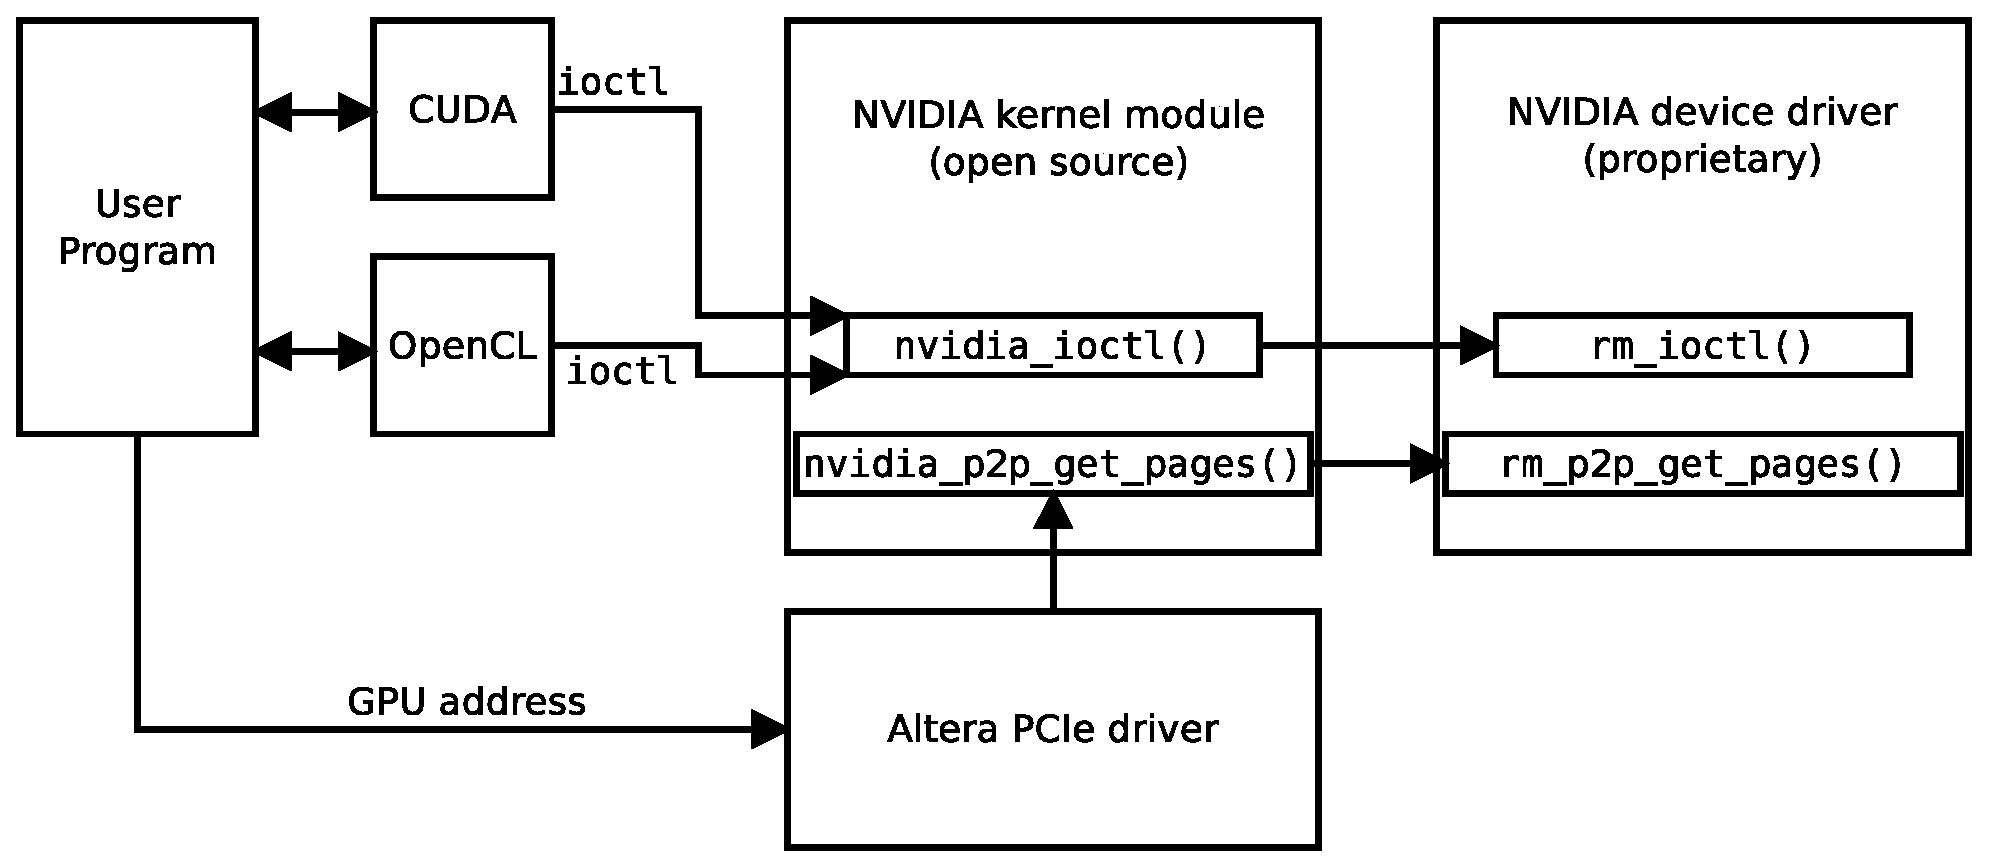
\includegraphics[width=0.9\textwidth]{images/ioctl_com.eps}}
	  \caption{Communication between CUDA/OpenCL and the NVIDIA driver}
	  \label{fig:ioctl_com}
\end{figure}


The GPUDirect RDMA function \texttt{nvidia\_p2p\_get\_pages} is defined in the NVIDIA kernel module and thus has itself no way of knowing whether CUDA or OpenCL is used in the user program.
As a consequence, there must be some differences in the way the two libraries communicate with the module.
Of special interest are the commands for buffer allocation.

%blackbox behaviour

In several experiments, the module has been modified to save all incoming \texttt{ioctl} commands and their parameter data to files on the hard drive to analyze them later.
Two minimalistic applications, one for CUDA and one for OpenCL, that perform as little initialization as needed and allocate one or more memory buffers provided the stimuli.
The data files were then compared for differences.

Some observations from the resulting data are that both libraries perform internal device memory management to some degree.
Small buffer allocations up to a size of 1MB are sometimes not relayed to the driver.
Additionally, NVIDIA's OpenCL implementation seems to utilize lazy buffer allocation, i.e. no communication to the driver happens until the buffer is actually used.
To circumvent this, at least one byte of data had to be written to the buffer for the experiments.

%TODO: in opencl: has to write at least a byte into the buffer
%175 ioctls just for init

The key finding from these experiments is that CUDA sends 3 \texttt{ioctl} messages to the kernel module to allocate a buffer, OpenCL on the other hand sends only 2.
Their request codes are as follows (command numbers highlighted):


\begin{center}
\begin{tabular}{| c | c | c |}
	\hline
	Order & CUDA & OpenCL\\
	\hline
	\hline
	1 & \texttt{0xc0a046{\bf\texttt4a}} &   \texttt{0xc0a046{\bf\texttt4a}}\\
	2 & \texttt{0xc03846{\bf\texttt57}} &   \texttt{0xc03846{\bf\texttt57}}\\
	3 & \texttt{0xc02046{\bf\texttt2a}} &    -\\
	\hline  
\end{tabular}
\end{center}



\emph{Libcudest} \cite{libcudest} is a project aimed at reverse engineering the CUDA platform.
Its documentation pages provide explanations to some of the command codes.
The \texttt{0x4a} and \texttt{0x57} commands are not listed but
the \texttt{0x2a} command, that is missing in OpenCL, is described there as a \emph{GPU method invocation}.
The \texttt{ioctl} parameter is 32 (\texttt{0x20}) bytes large and specifies the GPU method type in the second and third words, an address to the GPU method parameter in the fifth and sixth words and its size in the seventh and eighth words.
No information about the first word of the parameter is provided there.
The analysis of the data from several experiment trials showed that this word always contains the value \texttt{0xc1d00001} for the first process that is started after the NVIDIA driver is loaded.
It is then incremented for each following process that uses CUDA or OpenCL.
Therefore this word will be called \emph{User Identifier} in this thesis.
The following table provides an example of the \texttt{0x2a} \texttt{ioctl} parameter that is missing in OpenCL:

\begin{center}
\begin{tabular}{| c | c | l |}
	\hline
	%\multicolumn{2}{|c|}{parameter of \texttt{0x2a ioctl} command}\\
	Offset & Content & Description \\
	\hline
	\hline
	\texttt{0x00} & \texttt{0xc1d00001} &  \emph{User / Process Identifier} \\
	\hline
	\texttt{0x04} & \texttt{0x5c000007} &  GPU method type \cite{libcudest}\\
	\texttt{0x08} & \texttt{0x503c0104} &  \\
	\hline  
	\texttt{0x0c} & \texttt{0x00000000} &  unknown / always zero\\
	\hline
	\texttt{0x10} & \texttt{0xcbfe9bc0} &  Address to a GPU method parameter \cite{libcudest}\\
	\texttt{0x14} & \texttt{0x00007fff} &  (user space)\\
	\hline
	\texttt{0x18} & \texttt{0x00000004} &  Size of the GPU method parameter \cite{libcudest}\\
	\texttt{0x1c} & \texttt{0x00000000} &  (4 bytes)\\
	\hline
\end{tabular}
\end{center}

This GPU method (\texttt{0x5c000007:503c0104}) is not documented by Libcudest.
The GPU method parameter in this case is 4 bytes large.
Again, after data analysis it has been observed that, similarly to the User Identifier, this parameter value starts with a fixed number for the first device buffer allocation within a process and increments for each of the following buffer allocations.
It will be called \emph{Buffer Identifier} from now on.
For completeness, a GPU method parameter of the first user buffer allocated in CUDA is shown in this table:
\begin{center}
\begin{tabular}{| c | c | l |}
	\hline
	Offset & Content & Description \\
	\hline
	\hline
	\texttt{0x00} & \texttt{0x5c000029} & \emph{Buffer Identifier} \\
	\hline
\end{tabular}
\end{center}

%strace?

Both, the User Identifier as well as the Buffer Identifier are also present in the parameters of the preceding \texttt{0x4a} and \texttt{0x57} \texttt{ioctl} commands (also in OpenCL).
The following table shows a partial example of the \texttt{0x57} command parameter.
The identifiers are located at offsets \texttt{0x00} and \texttt{0x0c}.



\begin{center}
\begin{tabular}{| c | c | l |}
	\hline
	Offset & Content & Description \\
	\hline
	\hline
	\texttt{0x00} & \texttt{0xc1d00001} & \emph{User Identifier} \\
	\hline
	\texttt{0x04} & \texttt{0x5c000001} & {unknown} \\
	\hline
	\texttt{0x08} & \texttt{0x5c000003} & {unknown} \\
	\hline
	\texttt{0x0c} & \texttt{0x5c000029} & \emph{Buffer Identifier} \\
	\hline
	\texttt{0x10} & \texttt{0x00000000} & {unknown} \\
	\hline
	\texttt{0x14} & \texttt{0x00000000} & {unknown} \\
	\hline
	\texttt{0x18} & \texttt{0x04000000} & Buffer Size \\
	\texttt{0x1c} & \texttt{0x00000000} & (64MB) \\
	\hline
	\texttt{...} & \texttt{...} & {unknown} \\
	\hline
\end{tabular}
\end{center}

After sending the missing \texttt{0x2a} \texttt{ioctl} command with the correct identifiers manually, following to a call to \texttt{clCreateBuffer} in OpenCL, the \texttt{nvidia\_p2p\_get\_pages} will accept the OpenCL buffer and return its physical address.
This allows to emulate CUDA behavior in OpenCL for GPUDirect RDMA transfers.




\subsection{Extension of the NVIDIA Kernel Module}

\label{section:nvidiamod}

Neither the User Identifier nor the Buffer Identifier are accessible to the user application because they are managed internally by the CUDA and OpenCL libraries.
A possible way to retrieve them is to intercept the \texttt{0x4a} or \texttt{0x57} \texttt{ioctl} messages.
Again, modification of the NVIDIA kernel module is required.

The new module will simply extract the identifiers from the \texttt{0x57} messages and store them in a static variable.
A new \texttt{ioctl} command will then return the intercepted identifiers to the user application.
The the new request code should be chosen carefully, so that it does not collide with an existing NVIDIA \texttt{ioctl} command.
Unfortunately, a complete list of these codes is not available.
Out of observation and from the Libcudest project \cite{libcudest} the assumption was made that all original NVIDIA commands use read and write parameters as encoded in the bits 31 and 30 of the 32-bit request code.
In this case, the parameter can be write-only, thus the read bit has been chosen to be \texttt{0}.
At the same time, this should guarantee the new code to be collision-free.
Since two 32-bit values have to be retrieved, the parameter size (bits 29 to 16) should be \texttt{0x08}.
The module type code (bits 15 to 8) used by NVIDIA is \texttt{0x46} and was adopted.
Finally, the command number (bits 7 to 0) was chosen to be \texttt{0x00} resulting in the complete request code \texttt{0x40084600}.


%at least 1 MB buffers!

The changes applied to the module can be summarized as in listing \ref{listing:nvidia_mod}.

\begin{lstlisting}[label=listing:nvidia_mod, caption=Changes to \texttt{nvidia\_ioctl(..)} in the  NVIDIA kernel module]
if( arg_cmd == 0x57 )
{
	last_buffer_id = *(unsigned*)(arg_copy + 12);
	last_user_id = *(unsigned*)(arg_copy + 0);
}
if( cmd == 0x40084600 )
{
	((unsigned*)arg_copy)[0] = last_buffer_id;
	((unsigned*)arg_copy)[1] = last_user_id;
	goto done;
}
\end{lstlisting}

It should be noted that these modifications are not thread-safe, i.e. allocating multiple buffers in different threads or processes at the same time will cause race conditions.
However, since buffer allocation is usually performed only once during the initialization, this issue should not be of large concern.
Further development is needed if thread safety is desired.

%not threadsafe/multiprocess safe
%buffer allocation should not happen in multiple threads anyway
%only proof of concept..
%....more work is needed if this feature is desired












\section{User Space Invocation}
\label{section:userspace}

%small library: cl_rdma.c
A user space application cannot simply use the standard OpenCL data transfer functions to make use of the new capabilities of the modified driver.
Peer to peer transfer functions for example, are only provided by vendor specific extensions.
The small library \texttt{cl\_rdma.c} will thus provide an interface to the new RDMA mechanism.
An example minimal application is shown in appendix \ref{chapter:appendixA}.
This section is mainly concerned with the inner workings of this library.


The initialization procedure involves opening both of the device driver files located in the path \texttt{/dev/*}.
All of the communication to the drivers will happen will happen through the \texttt{read}, \texttt{write} and \texttt{ioctl} system calls on the resulting file descriptors.
An example of how to issue a command to the Altera driver, in this case the retrieval of the driver version, is shown in the listing \ref{userspaceinit}.
The modified driver appends the string \texttt{"with\_rdma"} to the version which should be checked to ensure that the correct driver is loaded.
Moreover, a signal handler has to be installed to catch the signals that are issued when a RDMA descriptor is finished.

%open /dev/acl0 file
\begin{lstlisting}[label=userspaceinit,caption=Initialization procedure]
//open the device drivers
int nvidia0fd = open( "/dev/nvidia0", O_RDWR );
int acl0fd = open( "/dev/acl0", O_RDWR );

//check whether the modified altera driver is loaded
char cbuf[1024] = { 0 };
struct acl_cmd cmd = { ACLPCI_CMD_BAR, ACLPCI_CMD_GET_DRIVER_VERSION,
                               NULL, &cbuf, sizeof(cbuf) };
read( acl0fd, &cmd, sizeof(cbuf) );
if( strstr( cbuf, "with_rdma" ) == NULL ){ return(1); }

//setup signal handler for interrupts from the driver
struct sigaction sa = { 0 };
sa.sa_sigaction = signal_handler;
sigemptyset( &sa.sa_mask );
sigaction( SIG_INT_RDMA, &sa, NULL );
\end{lstlisting}

The signal handler (listing \ref{signal_handler}) is very simple.
Its only task is to wake up the main thread which is waiting for a descriptor to complete.
This is done through a global semaphore.

\begin{lstlisting}[label=signal_handler,caption=Signal handler function]
static void signal_handler(int signum, siginfo_t* siginfo, void* uctx)
{
	sem_post( &semaphore );
}
\end{lstlisting}





\label{section:get_address}

An address from each buffer is needed for the RDMA transfers. Unfortunately, the OpenCL buffer allocation function \texttt{clCreateBuffer} returns an object of the type \texttt{cl\_mem} and not directly the address to the memory on the device.
In the header file \texttt{<CL/cl.h>}, the type \texttt{cl\_mem} is defined as
\begin{lstlisting}[label=kernel_get_address,caption=]
typedef struct _cl_mem* cl_mem;
\end{lstlisting}
with \texttt{struct \_cl\_mem} not defined, which means that the struct is defined externally in the proprietary NVIDIA or Altera OpenCL dynamic libraries and its layout is unknown.
Specifically, the buffer address cannot be simply extracted from the pointer.
A solution is to launch the kernel that is shown in listing \ref{kernel_get_address} with the desired buffer as parameter \texttt{a}.

\begin{lstlisting}[label=kernel_get_address,caption=OpenCL C kernel to retrieve the address from a \texttt{cl\_mem} object]
__kernel void get_address(__global unsigned long* a)
{
	a[0] = (unsigned long) a;
}
\end{lstlisting}

The kernel writes the address of the buffer into the buffer itself.
This value can then be retrieved by reading the first 8 bytes from the buffer with the \texttt{clEnqueueReadBuffer} function.
This procedure has to be performed only once for each buffer during the initialization of a program.


As noted in section \ref{section:cl_rdma}, normal NVIDIA OpenCL buffers cannot be simply pinned by the \texttt{nvidia\_p2p\_get\_pages} function.
The \texttt{0x2a} \texttt{ioctl} command has to be sent manually with the Buffer and User Identifiers retrieved from the modified NVIDIA module.
Moreover, the size of the buffer should be at least 1MB and one byte has to be written into it to ensure it is actually allocated.
The complete procedure is shown in listing \ref{pinnable_cl_buffer}

\begin{lstlisting}[label=pinnable_cl_buffer, caption=Creating a pinnable buffer in OpenCL]
//a buffer will not always be allocated if its smaller than 1MB
if( size < 1024 * 1024 ){	size = 1024 * 1024;	}
cl_mem buffer = clCreateBuffer(context,CL_MEM_READ_WRITE,size,NULL,NULL);

//make sure the buffer actually gets allocated by writing a byte into it
char dummydata = 0xff;
clEnqueueWriteBuffer(queue,buffer,CL_TRUE,0,1,&dummydata,0,NULL,NULL);

//get the buffer and user identifiers from the modified NVIDIA module
unsigned ioctl_param[2];
ioctl( fd, 0x40084600, ioctl_param );

//send the missing 0x2a ioctl to emulate CUDA behavior
unsigned gpu_method_param = ioctl_param[0];
unsigned gpu_method[8] = { ioctl_param[1],
                                    0x5c000007u,
                                    0x503c0104u,
                                    0x00000000u,
                                    0x00000000u,
                                    0x00000000u,
                                    0x00000004u,
                                    0x00000000u };
((unsigned long*) gpu_method)[2] = (unsigned long) &gpu_method_param;
ioctl( fd, 0xc020462a, gpu_method);
\end{lstlisting}










The actual transfer is started by sending the new \texttt{ACLPCI\_CMD\_RDMA} command to the Altera driver including the FPGA and GPU addresses.
This will invoke the function \texttt{rdma\_start} inside the driver.
As mentioned in section \ref{section:rdmaoverview}, the GPU is not able to pin more than ca. 200MB at a time.
Therefore, for large buffers, the transfer has to be partitioned into smaller blocks which are processed sequentially.
A rather small block size of 32MB was chosen.
This allows the look-up table (from the Lazy Unpinning optimization in section \ref{section:lazy}) to be used in a more efficient way: when frequent unpinning is required, only these 32 MB will be unpinned.
With a maximum size of 6, the table can thus hold up to 192MB pinned GPU blocks, which is almost the maximum amount that can be pinned at a time.
The block size of 32MB is still large enough to have no measurable impact on the performance.
%TODO: blocked 32MB transfers

\begin{lstlisting}[label=rdma_read,caption=RDMA transfer initation]
unsigned blocksize=1024*1024*32; //32MB
for(int i = 0; i < size; i += blocksize)
{
	if(i+blocksize> size){blocksize=size-i;}
	struct acl_cmd cmd={ACLPCI_DMA_BAR, ACLPCI_CMD_RDMA, 
		                  (void*)(fpga_address+i), (void*)(gpu_address+i),
		                   blocksize, 0};
	read(acl0fd, &cmd, blocksize);
	clrdma_wait_for_transfer(timeout_seconds);
}
\end{lstlisting}


As noted in section \ref{section:drivers}, kernel modules are always completely event-driven, i.e. do not have a main loop.
As a consequence, the RDMA component must be triggered from outside to continue with the transfer after a descriptor is finished.
%The hardware interrupt handler is not a suitable
This is done by sending the new driver command \texttt{ACLPCI\_CMD\_RDMA\_UPDATE} to the driver which will invoke the driver function \texttt{rdma\_update}.
To avoid busy waiting, a wait on a semaphore is used, which gets interrupted by the signal handler from listing \ref{signal_handler}.
In case of an error a timeout can be specified to avoid a deadlock.


\begin{lstlisting}[label=rdma_wait, caption=Driving the RDMA transfer]
struct timespec   ts;
struct timeval    tp;
gettimeofday(&tp, NULL);
// Convert from timeval to timespec
ts.tv_sec  = tp.tv_sec;
ts.tv_nsec = tp.tv_usec * 1000;
ts.tv_sec += timeout_seconds;

while(rdma_result != 0)
{
	//request transfer update from driver
	struct acl_cmd cmd={ACLPCI_DMA_BAR, ACLPCI_CMD_RDMA_UPDATE, 
	                           NULL, NULL, 0};
	rdma_result=read(acl0fd, &cmd, sizeof(cmd));
	if(rdma_result == 0){ break; } //transfer done
	
	//wait for interrupt from signal handler
	while(1)
	{
		int rc=sem_timedwait(&semaphore, &ts);
		if(rc && errno == EINTR){ continue; } //spurious wakeup
		else{ break; } //actual interrupt or timeout	} }
\end{lstlisting}






		
		\chapter{Implementation of Concurrent Indirect GPU-FPGA Communication}
\label{section:concurrent}

While direct device to device communication is in theory always the fastest possible method, it is more cumbersome to use, requires unofficial modified drivers and is only available for NVIDIA Quadro and Tesla graphics cards.
The indirect method that involves a round-trip via the CPU on the other hand can be simply implemented in standard OpenCL, also with the more popular GeForce cards.
This section describes a naive version and an optimization that can be applied for large transfers

The simplest possible procedure of an indirect transfer can be summarized as follows:
\begin{enumerate}
	\item Read data from the first device into a CPU buffer
	\item Wait until the transfer is done
	\item Send data from the CPU buffer to the second device
\end{enumerate}

In OpenCL this can easily be accomplished in only two lines of code (error checking omitted):
%TODO: code listing
\begin{lstlisting}[label=sequential_indirect,caption=Sequential indirect device to device transfer in OpenCL]
clEnqueueReadBuffer (queue_device1, buffer_device1, CL_TRUE, 
                            0, size, cpu_buffer, 0, NULL, NULL);
clEnqueueWriteBuffer(queue_device2, buffer_device2, CL_TRUE, 
                            0, size, cpu_buffer, 0, NULL, NULL);
\end{lstlisting}

However, this is highly inefficient because at any time one of the two devices is not doing anything.

Both, the GPU as well as the FPGA have one DMA controller.
Both can operate independently of each other.
By splitting up a large transfer into multiple small transfers, one DMA controller can read from a portion of the temporary CPU buffer while the other one is simultaneously writing to the next portion.
This results in an overall faster transfer, as illustrated in figure \ref{fig:concurrent1}.


\begin{figure}[htb]
	  \centerline{
		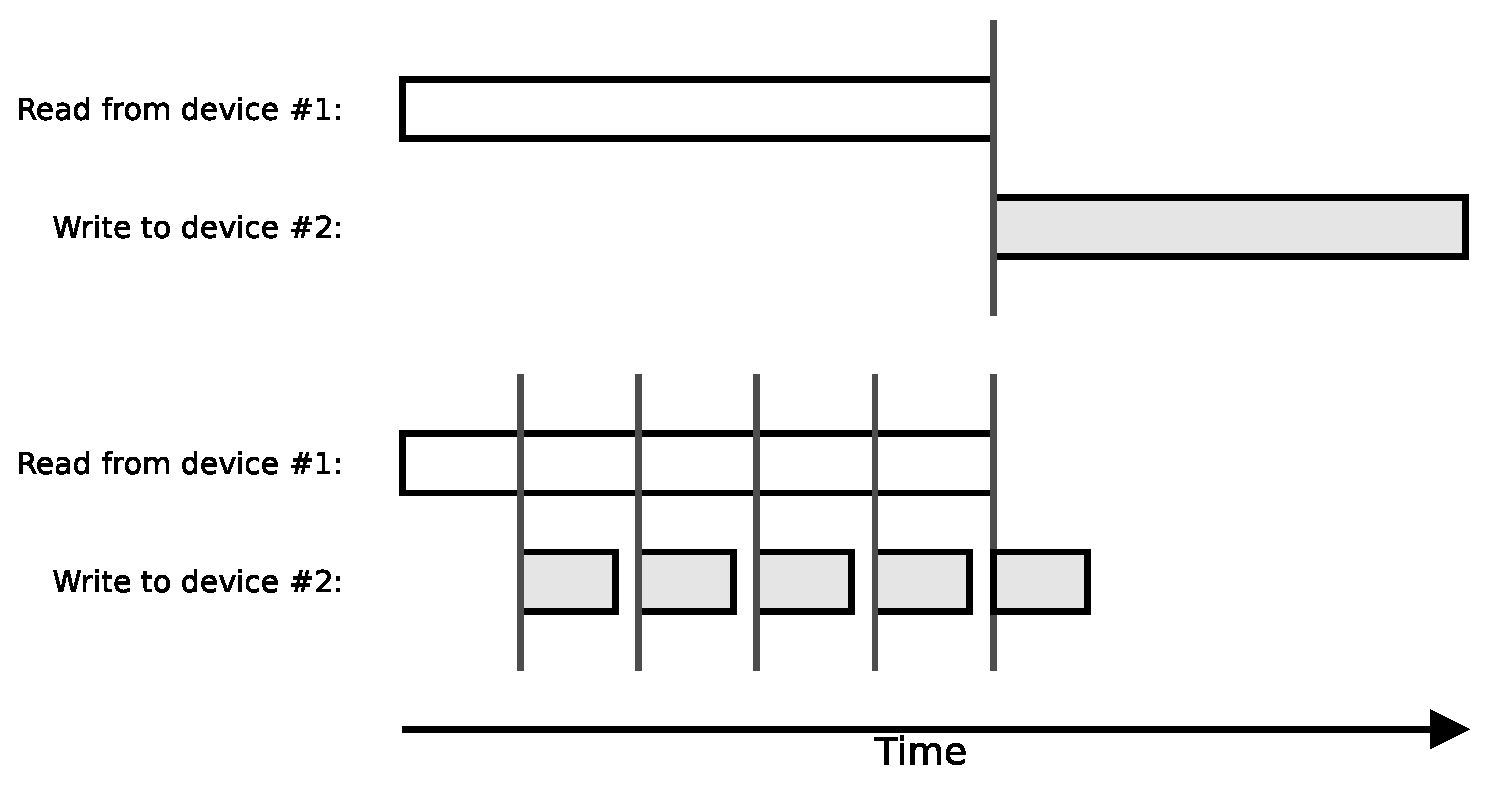
\includegraphics[width=1.0\textwidth]{images/concurrent1.eps}}
	  \caption{Comparison of sequential (top) and concurrent (bottom) indirect transfer strategies. The two large transfers are splitted into 10 smaller transfers, 8 of them can be performed simultaneously. The gray vertical lines represent synchronization barriers.}
	  \label{fig:concurrent1}
\end{figure}


An important parameter is the size and number of the smaller transfers.
If their size is too large, hardly any benefit from the concurrency is gained.
With a lot of transfers on the other hand, too much time is wasted for synchronization and in the worst case may be even slower than the sequential transfer strategy.
%not too large not too small
Different parameters were evaluated and the results are presented in section \ref{sec:results_concurrent}.


During the implementation of this transfer strategy, several problems appeared that are documented in the following paragraphs:

The first attempt was to utilize the \emph{asynchronous} memory transfer capabilities of OpenCL.
A function call that initiates an asynchronous transfer does not wait until the transfer is done and returns immediately.
This can be used to perform other operations in the meantime.
In OpenCL, the \texttt{blocking\_write} argument of the \texttt{clEnqueueWriteBuffer} can be set to \texttt{CL\_FALSE} to start an asynchronous write operation.
The complete but simplified code is presented in listing \ref{async_indirect} (error checking omitted).

\begin{lstlisting}[label=async_indirect,morekeywords={CL_TRUE, CL_FALSE},caption= Asynchronous indirect device to device transfer]
unsigned bytes_done = 0;
while(bytes_done < size)
{
	if(blocksize > size - bytes_done ){blocksize = size - bytes_done;}
	
	//synchronous read
	clEnqueueReadBuffer (queue_device1, buffer_device1, CL_TRUE, 
	                            bytes_done, blocksize, cpu_buffer+bytes_done,
	                            0, NULL, NULL);
	//asynchronous write
	clEnqueueWriteBuffer(queue_device2, buffer_device2, CL_FALSE, 
	                            bytes_done, blocksize, cpu_buffer+bytes_done,
	                            0, NULL, NULL);
	bytes_done += blocksize;
}
//wait for the asynchronous write transfers to finish
clFinish(queue_device2);
\end{lstlisting}

The first observation from the execution of this code was, that NVIDIA's implementation of the \texttt{clEnqueueWriteBuffer} function does not return immediately despite passing \texttt{CL\_FALSE} as the \texttt{blocking\_write} argument. 
Instead it blocks until the write is completed, as if it was a synchronous transfer.
The solution to this issue can be found in the \emph{NVIDIA OpenCL Best Practices Guide} \cite{nvidia_cl_best_practices}.
A \emph{pinned} CPU memory buffer is required as the source for asynchronous writes.
It can be created as shown in listing \ref{pinned_opencl} and simply used in the previous code example.

\begin{lstlisting}[label=pinned_opencl,morekeywords={}, caption= Creation of a pinned CPU buffer in OpenCL]
cl_mem pinned_buffer =
    clCreateBuffer(gpu_context, 
                        CL_MEM_READ_ONLY | CL_MEM_ALLOC_HOST_PTR, 
                        size, NULL, NULL);

unsigned char* cpu_buffer = 
    (unsigned char*) clEnqueueMapBuffer(gpu_queue, pinned_buffer, CL_TRUE, 
                                                    CL_MAP_WRITE, 0, size, 0,
                                                    NULL, NULL, NULL); 
\end{lstlisting}


The larger issue stems from the Altera side.
Though its asynchronous transfer initiation call does not block (as expected), the \texttt{clFinish} function, required for the final synchronization, blocks for a surprisingly long time.
In fact, this time is roughly equivalent to the time that is needed for a complete synchronous transfer.
This indicates that no data is actually transferred, until this function is called.
This suspicion is substantiated when taking into account the architecture of the Altera PCIe driver:
Its DMA component does not notify the user space process when a transfer (or a portion of it) is completed.
Instead, it relies on \emph{polling} from the user space to drive the transfer.
In all likelihood this polling is performed by \texttt{clFinish}.

In an attempt to circumvent this problem, the code has been modified to start a second thread which calls the \texttt{clFinish} function while the main thread continues to issue the asynchronous transfers as before.
%This second thread drives the transfer
Though at first glance, this seemed to work, a new unexpected behavior appeared:
Approximately 2\% of the time, \texttt{clFinish} did not terminate at all (or resulted in a segmentation fault after some time) while CPU usage was constantly at 100\% workload.
This behavior is of course not acceptable in a real application.
The reasons for this are unknown.
One can only speculate that Altera's OpenCL implementation is maybe not thread-safe.

The final solution that proved to work, was to use only synchronous transfers, but in two threads.
While one thread is only concerned with reading from device 1, the second thread waits until a read transfer is finished and then performs a blocking write to device 2.
The simplified code for both threads is shown in listings \ref{concurrent_read_thread} and \ref{concurrent_write_thread}.

\newpage

\begin{lstlisting}[label=concurrent_read_thread,morekeywords={}, caption= First thread for concurrent device to device transfer]
unsigned bytes_read = 0;
pthread_t write_thread;
pthread_create( &write_thread, NULL,
                     concurrent_write_thread, (void*) &bytes_read);
while(bytes_read < size)
{
	clEnqueueReadBuffer(queue_device1, buffer_device1, CL_TRUE,
	                           bytes_read, blocksize, cpu_buffer+bytes_read,
	                           0, NULL, NULL);
	
	bytes_read += blocksize;
}
pthread_join(write_thread, NULL);
\end{lstlisting}


\begin{lstlisting}[label=concurrent_write_thread,morekeywords={bytes_read}, caption= Second thread for concurrent device to device transfer]
unsigned bytes_sent = 0;
while(bytes_sent < size)
{
	//busy waiting until a read transfer is completed
	while(bytes_sent >= bytes_read)	{	sched_yield();	}
	
	clEnqueueWriteBuffer(queue_device2, buffer_device2, CL_TRUE,
	                            bytes_sent, blocksize, cpu_buffer+bytes_sent,
	                            0, NULL, NULL);
	
	bytes_sent += blocksize;
}
\end{lstlisting}



Note that no synchronization with mutexes is required to access the shared  variable \texttt{bytes\_read} because this is a \emph{single producer single consumer} case.
However, a condition variable may be useful to eliminate the busy waiting loop.
Additionally for stability reasons, an \emph{abort flag} is shared between the threads, not shown in these code snippets.


		
		\chapter{Evaluation}
\label{sec:results}

The three methods (direct, concurrent indirect and sequential indirect) have been evaluated for bandwidth.
This section presents the results of these evaluations.
All tests were performed 5 times and the results averaged.
In each trial, the memory buffer on the first device was filled with random data.
After the benchmarked transfer from device 1 to device 2, the data was read out from the second device again and compared to the original data to make sure it is correct.

The largest issue that appeared already during the development of the driver is that the direct transfer in the direction from the GPU to the FPGA does not work.
Trying this direction, will make the FPGA board unresponsive or may even result in a complete freeze of the operating system.
This makes the issue hard to debug, because each time a system reboot is required.
Despite extensive efforts, including an analysis of the OpenCL IP system on the FPGA and contacting Altera, this issue could not be fixed during this thesis.



\section{Hardware Configuration}
%stratix v nallatech
%quadro 
%#of pcie lanes
%CPU-Device transfer speed
%driver versions
%amount of memory / type of memory? GDDR?

A NVIDIA Quadro GPU and an Altera Stratix V FPGA were used for the development and evaluation during this thesis.
The relevant features for both devices are shown in the following table:

\begin{center}
\begin{tabular}{| l | c | c |}
	\hline
	 & FPGA \cite{nallatech385} & GPU \cite{quadrok600}\\
	\hline
	\hline
	Model & Nallatech 385-D5 & Hewlett-Packard Quadro K600\\
	\hline
	Architecture & Altera Stratix V D5 & NVIDIA Kepler GK 107\\
	\hline
	Original driver version & 13.1 & 340.58 \\
	\hline
	PCIe Generation & 3.0  & 2.0 \\
	\hline
	Number of PCIe lanes & 8x  & 16x \\
	\hline
	Global memory size & 8GB  & 1GB \\
	\hline
	Memory type & DDR3  & GDDR3 \\
	\hline
	Measured bandwidth to CPU & 750 MB/s & 1930 MB/s\\
	\hline
	Measured bandwidth from CPU & 550 MB/s & 1950 MB/s\\
	\hline
\end{tabular}
\end{center}




\section{Effects of RDMA Optimizations} 

To  find out to which extent the optimizations from section \ref{sec:optimizations} contribute to the final performance, each of them has been evaluated.
The results are shown in figure \ref{fig:optimizations_eval}.

The first version, that was developed mainly as a prototype performs very poorly, as expected.
A maximum bandwidth of only 170 MB/s has been measured, which is even slower than the sequential indirect transfer method.
Its main bottleneck is the response latency from a PCIe interrupt until the next descriptor is sent, as indicated by the measurements from the larger descriptors optimization.
This optimization had the largest impact, raising the bandwidth to ca. 580 MB/s for large transfers with 512KB descriptor sizes.


The multiple descriptors optimization raises the maximum measured bandwidth to ca. 610 MB/s.
The overall improvement is rather small because of the limitation of being able to process only 2 descriptors at a time which in turn is due to the small ATT.

Lazy unpinning contributes a roughly constant performance gain, independent of the transfer size.
This is especially important for the smaller transfers.
Note that the data for this version does not include the first transfer, which performs the actual pinning and does not benefit from this optimization.
Only the subsequent transfers are considered.
This is nevertheless representable, since real applications usually require many transfers.

\begin{figure}[htb]
	  \centerline{
		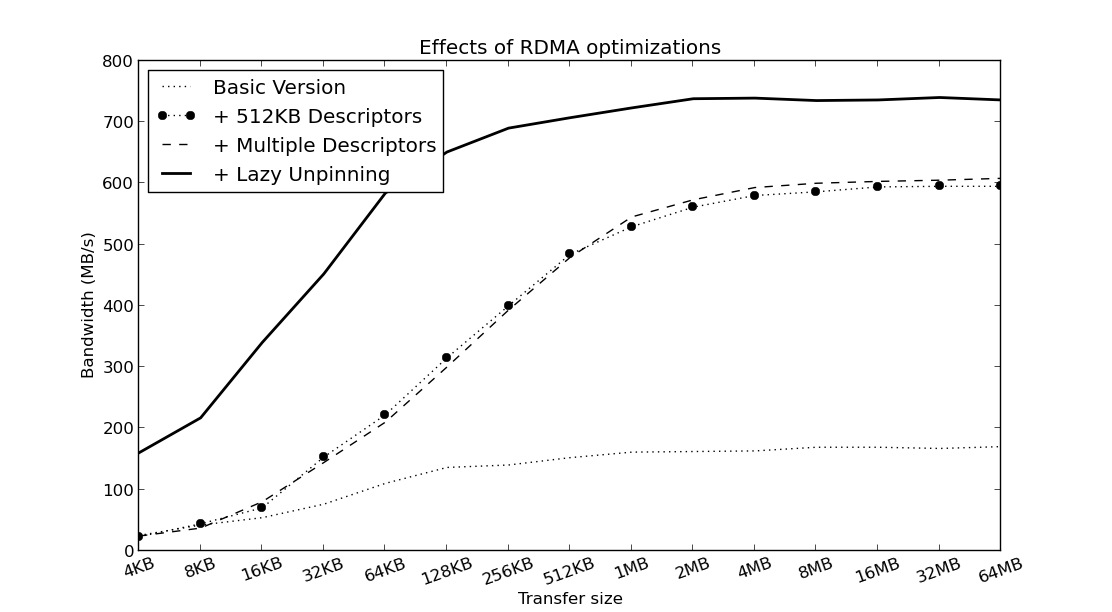
\includegraphics[width=1.3\textwidth]{images/optimizations_eval2}}
	  \caption{Comparison of the optimizations described in section \ref{sec:optimizations}. Each optimization is added to the previous version (i.e. the Lazy Unpinning benchmark also includes the Multiple Descriptors and 512KB Descriptors optimizations). The Lazy Unpinning benchmark does not include the first transfer, which performs the actual memory pinning.}
	  \label{fig:optimizations_eval}
\end{figure}


\section{Parameter Choice for Concurrent Indirect Transfer}
\label{sec:results_concurrent}

As already mentioned in section \ref{section:concurrent}, the choice of the block size parameter is important for the concurrent indirect transfer method.
Different values have been evaluated. Figure \ref{fig:results_blocksizes} presents the results.

The preliminary idea that too small and too large block sizes are detrimental can be confirmed.
However, the extent partly depends on the transfer size and direction.
For the direction from the GPU to the FPGA, a block size of one fourth of the transfer size seems to be an overall good choice.
The opposite direction is not as clear.
Large transfers seem to benefit from smaller block sizes of ca. one eighth of the overall size, whereas for small transfers the synchronization costs are rather large and a blocks of one half of the overall size should be chosen.


\begin{figure}[h]
\begin{center}$
\begin{array}{cc}
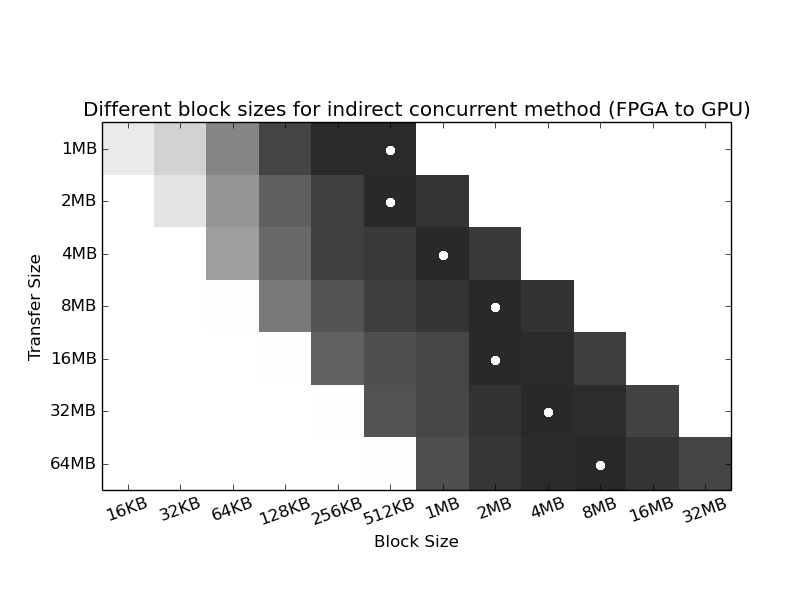
\includegraphics[height=0.45\textheight]{images/fg_dots.png} \\
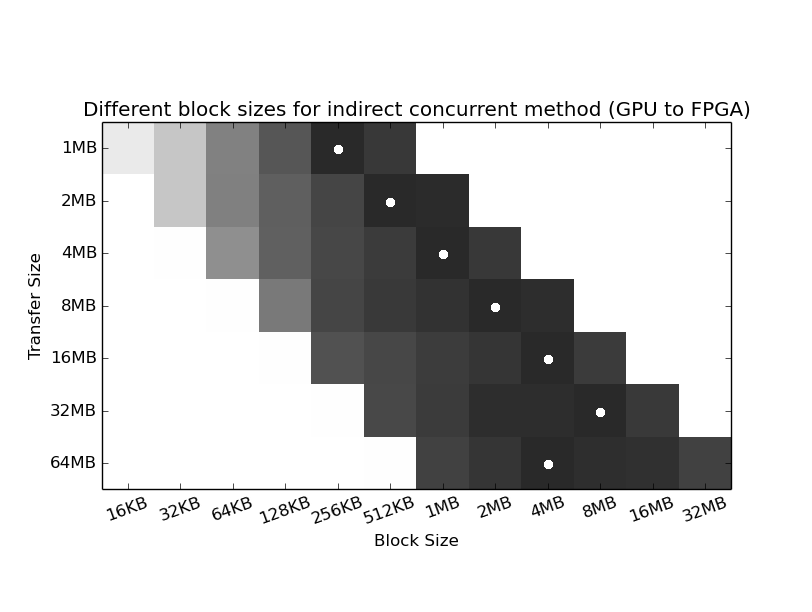
\includegraphics[height=0.45\textheight]{images/gf_dots.png}
\end{array}$
\end{center}
\caption{Influence of the block size parameter on the performance for the concurrent indirect transfer method. Higher bandwidth is darker. The white dots mark the maximum bandwidth for each transfer.}
\label{fig:results_blocksizes}
\end{figure}


%TODO: bar plot of five transfers that shows lazy unpinning effect?



\section{Method Comparison}

Figure \ref{fig:results_comparison} presents a comparison of the sequential indirect, concurrent indirect and the direct transfer methods.
For contrast, the CPU-FPGA bandwidth, which can be regarded as an upper limit for the GPU-FPGA bandwidth, is also shown.
Again, the first transfer which includes the expensive pinning operation is not included in the graphs.

Different block size values were used for the concurrent indirect method:
Transfers with sizes until including 1MB used a value of one half, from 2MB until 8MB a value of one fourth and from 16MB on a value of one eighth  of the overall size.

As expected, the direct transfer method is indeed the fastest of the three methods, peaking at 740MB/s.
For large transfers the concurrent indirect approach performs almost as well with a speed of up to 730MB/s.
This results in a speed-up of ca 30\% and 28\% compared with the indirect transfers.
For the direction from the GPU to the FPGA, for which the direct transfer could not be enabled, this is even the best solution, with a bandwidth of ca 525MB/s and a speed-up of ca 39\%.



The bandwidth of the direct method deteriorates after the 192MB transfer size mark.
This is due to the limitation of the graphics card not being able to pin more than ca. 200MB at a time.
For larger transfers, a memory region has to be unpinned first which costs a significant amount of time.

The 512MB transfer for the concurrent indirect method failed to succeed.
Presumably, the pinned CPU memory buffer (mentioned in section \ref{section:concurrent}) uses up space not only on the CPU but also on the GPU.
As a consequence this exceeds the memory limit of the Quadro K600 of 1GB.


%first transfer not included because of pinning


\begin{figure}[h]
\begin{center}
$
\begin{array}{cc}
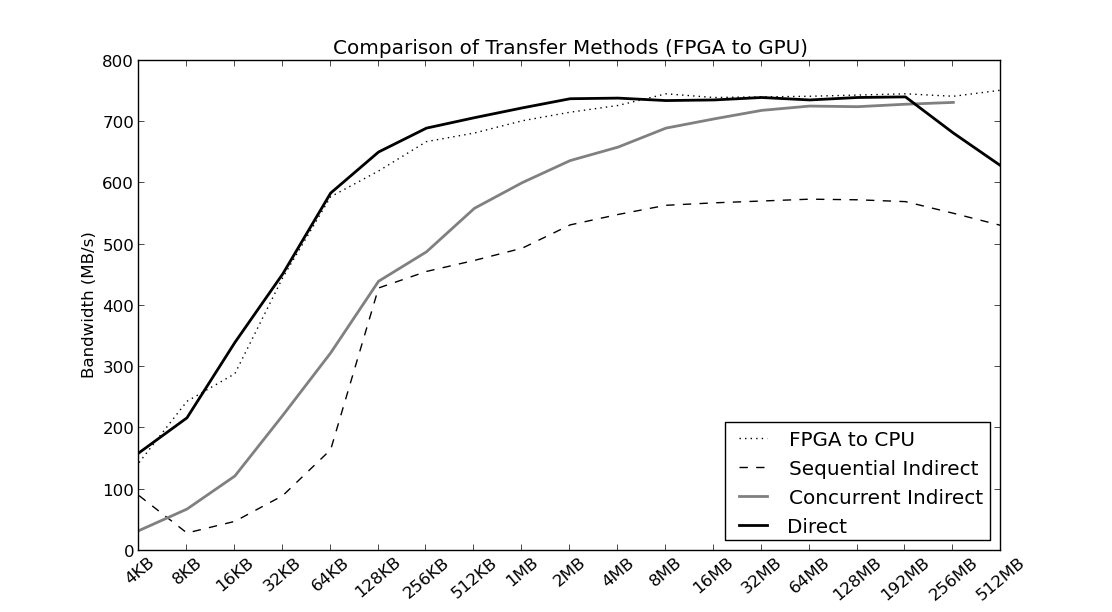
\includegraphics[height=0.41\textheight]{images/results_comp1.png} \\
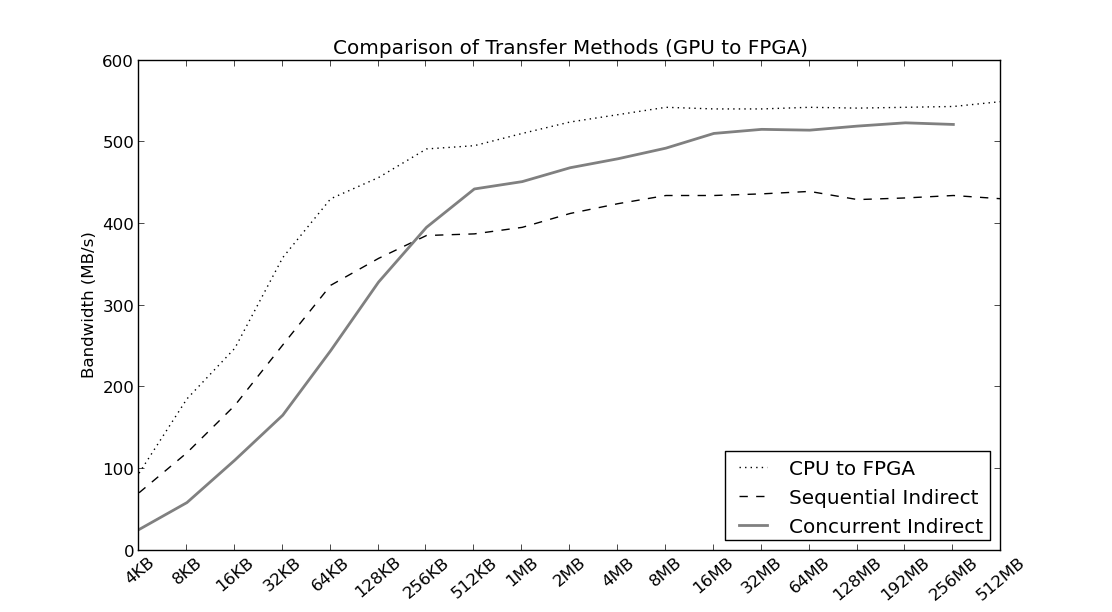
\includegraphics[height=0.41\textheight]{images/results_comp2.png}
\end{array}
$
\end{center}
\caption{Comparison of sequential indirect, concurrent indirect and direct transfer methods.}
\label{fig:results_comparison}
\end{figure}




\section{Comparison with Previous Work}
\label{section:previousworkcomparison}

The following table compares the relevant features of the approaches from previous research, presented in section \ref{section:previouswork} and the two approaches from this thesis, direct and concurrent indirect (the two columns on the right).
Note that the bandwidths cannot be simply compared due to different devices.


\begin{center}
\begin{tabular}{| l || c| c |c|| c | c |}
	\hline
		&	\multicolumn{3}{c||}{Previous Work} & \multicolumn{2}{c|}{This Thesis}\\
	\hline
		&	Bittner \& Ruf & FPGA$^2$ & Susanto & Direct & Concurrent\\
	\hline\hline
	Operating System & Windows & Linux & Linux & \multicolumn{2}{c|}{Linux}\\
	\hline
	DMA Master & GPU & FPGA & FPGA & FPGA & Both \\
	\hline
	Processes & 1 & 1 & 2 & \multicolumn{2}{c|}{1}\\
	\hline
	FPGA Vendor & Xilinx & Xilinx & Altera & \multicolumn{2}{c|}{Altera}\\
	\hline
	FPGA Model & Virtex 6 & Virtex 5 & Stratix V & \multicolumn{2}{c|}{Stratix V}\\
	\hline
	FPGA IP Stack & Custom & Custom & Vendor & \multicolumn{2}{c|}{Vendor} \\
	\hline
	FPGA Driver & Custom & Custom & Modified & Modified & Original\\
	\hline
	FPGA Programming & HDL & HDL & OpenCL & \multicolumn{2}{c|}{OpenCL}\\
	\hline
	GPU Vendor & NVIDIA & NVIDIA & NVIDIA & \multicolumn{2}{c|}{NVIDIA}\\
	\hline
	GPU Model & GeForce& GeForce & GeForce & \multicolumn{2}{c|}{Quadro}\\
	&  GTX580 & 8400GS & GTX660Ti &  \multicolumn{2}{c|}{K600}\\
	\hline
	GPU Driver & Original & Nouveau & Original & Modified & Original \\
	\hline
	GPU Programming & CUDA & gdev & CUDA & \multicolumn{2}{c|}{OpenCL}\\
	\hline
	Effective PCIe lanes & 8 & 1 & 8 & \multicolumn{2}{c|}{8}\\
	\hline
	Effective & 1.0 & 1.1 & not & \multicolumn{2}{c|}{2.0}\\
	PCIe generation & & & specified & \multicolumn{2}{c|}{} \\
	\hline
	\hline
	Maximal bandwidth & 514MB/s & 203MB/s & 680MB/s & 740MB/s & 730MB/s\\
	FPGA to GPU & & & & &\\
	\hline
	Maximal bandwidth & 1.6GB/s & 189MB/s & 540MB/s & N/A & 525MB/s\\
	GPU to FPGA & & & & &\\
	\hline
\end{tabular}
\end{center}

The approaches that utilize the FPGA as the DMA master perform better for the direction from the FPGA to the GPU.
The opposite is true if the GPU is used as the DMA master.
This may have to do with the PCIe protocol: an extra PCIe packet is required to read from another device, whereas writing to the other device requires only one packet.




		
		\chapter{Conclusions and Future Work}
\label{section:conclusions}

This thesis shows an example implementation of direct communication between a GPU and a FPGA over PCIe for use in OpenCL.
Several major problems had to be solved, e.g. the lack of official support of the GPUDirect RDMA technology for OpenCL and the lack of an ICD from Altera.
Unfortunately, only the transfer direction from FPGA to GPU could be realized.
This direction showed significant performance improvement compared to the indirect method with a round-trip via CPU.
Moreover, an alternative to the direct method, that is simple to implement yet yields decent results and works for both directions, has been evaluated.

%summary

Several enhancements, that either could not be finished in time or go beyond the scope of this thesis, are still imaginable:

%-real application
%-investigate the reasons why GPU-to-FPGA direction fails.

\begin{itemize}
\item The largest drawback of the implemented method is that the GPU-to-FPGA direction could not be enabled.
Further investigation is required to find out the reasons why this direction fails.
A possible approach may include a thorough analysis of the OpenCL Verilog code provided by Altera.
\item The Installable Client Driver that was implemented for Altera OpenCL during the practical part of this thesis is still incomplete as it only wraps the most basic OpenCL functions.
But also those that were implemented lack the support for OpenCL events, which can be useful for asynchronous transfers.
Supporting events would require a rather complicated memory management system that keeps track of the event objects' lifetimes.
The development of a full ICD is more time consuming than could be achieved during this thesis.
However, Altera announced a full ICD implementation in the upcoming SDK version 15.0.

\item The GPUDirect RDMA technology that was used as the basis for direct GPU-FPGA communication is only available for the NVIDIA Quadro and Tesla graphics cards.
A possible alternative is to utilize a similar approach as Bittner and Ruf, which is described in section \ref{bittner}, however without their Speedy PCIe IP core.
In theory, its functionality can be provided by the Altera's PCIe driver and PCIe core.
In contrast to this thesis which utilizes the DMA controller on the FPGA, this alternative would employ the GPU's DMA controller.
Not only may this enable the direct communication also for the popular GeForce cards but also the still missing GPU-to-FPGA direction.

\item It may be interesting see to which extent the higher bandwidth will speed up an existing application that uses a heterogeneous computing system employing GPUs and FPGAs.
A candidate could be the lane detection algorithm for automated driving, used at the TU Munich \cite{lanedetection} or some of the examples provided in \cite{chimera}.



\end{itemize}

%TODO: find out why direct write to fpga fails: maybe analze verilog/vhdl
% test with a real life application






		
		% ---------------------------------------------------------------------------
		%
		% Appendix
		%
		% ---------------------------------------------------------------------------
		
		\part*{Appendix}
		\addcontentsline{toc}{part}{Appendix}
		
		\appendix %---------------------------------------
		
		\chapter{Simulation Parameters}

%\section{Detailed Validation Results}

\label{chapter:appendixA}

\begin{center}
	\begin{tabular}{| c | c |}
		\hline
		\_Q\_lr & 0.001 \\
		\_action\_l2 & 1.0 \\
		\_batch\_size & 256 \\
		\_buffer\_size & 1000000 \\
		\_clip\_obs & 200.0 \\
		\_hidden & 256 \\
		\_layers & 3 \\
		\_max\_u & 1.0 \\
		\_network\_class & baselines.her.actor\_critic:ActorCritic \\
		\_norm\_clip & 5 \\
		\_norm\_eps & 0.01 \\
		\_pi\_lr & 0.001 \\
		\_polyak & 0.95 \\
		\_relative\_goals & False \\
		\_scope & ddpg \\
		aux\_loss\_weight & 0.0078 \\
		bc\_loss & 0 \\
		demo\_batch\_size & 128 \\
		gamma & 0.98 \\
		n\_batches & 40 \\
		n\_test\_rollouts & 10 \\
		noise\_eps & 0.2 \\
		num\_demo & 100 \\
		prm\_loss\_weight & 0.001 \\
		q\_filter & 0 \\
		random\_eps & 0.3 \\
		replay\_k & 4 \\
		replay\_strategy & future \\
		rollout\_batch\_size & 2 \\
		test\_with\_polyak & False \\
		\hline
	\end{tabular}
\end{center}




		\chapter{Setup Instructions}

\label{chapter:appendixB}

%TODO DELETE

This section provides an overview of the procedures needed to run the benchmarks from the source code package included for this thesis.
The Ubuntu 14.04 OS is assumed.


The following commands install the Altera ICD on the system:
\begin{lstlisting}[label={}, caption={}]
sudo mkdir /etc/OpenCL/AlteraICD
sudo cp -r altera_icd/bin/* /etc/OpenCL/AlteraICD
sudo sh -c "echo '/etc/OpenCL/AlteraICD/libalteraicd.so.1' \
     >> /etc/OpenCL/vendors/altera.icd"
\end{lstlisting}

The modified Altera PCIe module can be compiled with the following script:
\begin{lstlisting}[label={}, caption={}]
./make_all.sh
\end{lstlisting}

The modified NVIDIA module can be compiled with the following command:
\begin{lstlisting}[label={}, caption={}]
make module
\end{lstlisting}

To load the modified modules, the original modules have to be removed first.
Since the display manager depends on the NVIDIA module it must be stopped too.
To do this, the TTY has to be switched, e.g. with the key combination \texttt{CTRL+ALT+F4}.
Then, the following command sequence will replace the modules:
\begin{lstlisting}[label={}, caption={}]
sudo service lightdm stop
sudo rmmod nvidia-uvm aclpci_drv nvidia
sudo insmod nvidia.ko
sudo insmod aclpci_drv.ko
sudo service lightdm start
\end{lstlisting}

To load the modules automatically during the boot procedure, the previous modules should be overwritten:
\begin{lstlisting}[label={}, caption={}]
sudo cp aclpci_drv.ko /lib/modules/$(uname -r)/misc/
sudo cp nvidia.ko /lib/modules/$(uname -r)/kernel/drivers/
\end{lstlisting}

For testing, the code from appendix \ref{chapter:appendixA} or the provided benchmark \texttt{direct\_benchmark} can be used.



		
	


  \clearemptydoublepage

	\bibliography{bibliography/literature}
	

\end{document}

